\documentclass[journal]{IEEEtran}

\usepackage{cite}
\usepackage{amsmath,amssymb,amsfonts}
\usepackage{algorithmic}
\usepackage{graphicx}
\usepackage{textcomp}
\usepackage{xcolor}
\usepackage{booktabs}
\usepackage{multirow}
\usepackage{url}
\usepackage{hyperref}
\usepackage{caption}
\graphicspath{{../figures/}}

\begin{document}

\title{A Reproducible, Fairness-Aware, and Explainable Machine Learning Framework for Credit Risk Scoring: Evidence from the Home Credit Default Risk Dataset}

\author{
\IEEEauthorblockN{Author Name\IEEEauthorrefmark{1}}
\IEEEauthorblockA{\IEEEauthorrefmark{1}Affiliation to be completed by author, Department/Institution, City, Country\\
Email: ahamril2265@gmail.com}
}

\markboth{Preprint, prepared for submission to an applied machine learning / financial analytics journal, 2026}{}

\maketitle

\begin{abstract}
Credit risk scoring is a foundational task in consumer lending, where a lender must estimate the probability that an applicant will default on a loan and translate that estimate into an actionable, auditable decision. This paper presents a complete, reproducible pipeline for credit risk scoring built on the Home Credit Default Risk dataset (307,511 applicants, seven relational tables). The pipeline integrates domain-driven feature engineering, correlation- and variance-based feature filtering, Principal Component Analysis (PCA) for dimensionality reduction (207 engineered features reduced to 119 components retaining 95\% of variance), and seven supervised classifiers (Logistic Regression, Decision Tree, $K$-Nearest Neighbors, Gaussian Naïve Bayes, Random Forest, XGBoost, and LightGBM), each evaluated in both a default-hyperparameter baseline configuration and a hyperparameter-optimized (tuned) configuration. Beyond standard accuracy-oriented reporting, the framework contributes: (i) probability calibration via Platt scaling and isotonic regression; (ii) SHapley Additive exPlanations (SHAP) for five of the seven model families; (iii) paired statistical significance testing (McNemar's test and DeLong's test) between the two top-ranked models; (iv) an extended metric suite robust to class imbalance (Matthews Correlation Coefficient, Cohen's Kappa, Average Precision, and the Kolmogorov--Smirnov statistic); (v) a battery of fairness diagnostics (demographic parity, disparate impact ratio, equal opportunity, and equalized odds) across gender, income type, and education level; and (vi) three exploratory contributions --- cost-sensitive threshold optimization, bootstrap feature-stability analysis, and a direct PCA-versus-non-PCA benchmark. After hyperparameter optimization and calibration, a tuned Logistic Regression model attains the highest ROC-AUC (0.7583) on a held-out test set of 61,503 applicants, statistically indistinguishable from the runner-up, LightGBM (McNemar $p=0.29$; DeLong $p=0.57$), while offering superior computational efficiency and regulatory interpretability. Predicted probabilities are converted into a standardized 300--900 credit score, and applicants are stratified into five interpretable risk bands. All code, trained models, figures, and result tables are version-controlled and reproducible under a fixed random seed. We report all findings --- including a substantial PCA-versus-non-PCA performance gap attributable to feature scaling sensitivity, and a data-driven limitation of the fairness diagnostics arising from small demographic subgroup sizes --- transparently, consistent with the goal of producing a scientifically honest, deployment-aware credit scoring artifact rather than an idealized one.
\end{abstract}

\begin{IEEEkeywords}
credit risk scoring, machine learning, explainable AI, SHAP, algorithmic fairness, probability calibration, hyperparameter optimization, principal component analysis, statistical model comparison, financial analytics.
\end{IEEEkeywords}

\section{Introduction}

Consumer lending institutions rely on credit risk models to estimate the probability that a loan applicant will fail to repay an extended line of credit. These estimates directly determine loan approval, pricing, and portfolio risk exposure, and are therefore subject to increasing scrutiny from regulators (e.g., the Equal Credit Opportunity Act in the United States, and the EU AI Act's classification of credit scoring as a ``high-risk'' AI application). A modern credit risk scoring system must therefore satisfy three simultaneous, and at times competing, requirements: (1) strong discriminative \emph{predictive performance}; (2) \emph{interpretability}, so that adverse decisions can be explained to applicants and regulators; and (3) demonstrable \emph{fairness} across protected demographic groups.

The majority of published credit scoring studies report a single point estimate of predictive accuracy (typically ROC-AUC) for a handful of candidate algorithms and treat the highest-scoring model as the de facto ``best'' choice, without testing whether the performance gap between the top candidates is statistically distinguishable from noise, without calibrating the reported probabilities, and often without any fairness auditing at all. This gap between academic reporting practice and the requirements of a deployable, auditable financial system motivates the present work.

This paper documents an end-to-end credit risk scoring pipeline developed on the Home Credit Default Risk dataset, a large, publicly available, multi-table dataset representative of the data an actual lender would hold (application-level demographic and financial data, credit bureau history, prior application history, point-of-sale and credit-card balance histories, and installment repayment history). Rather than treating model selection as the terminal step, we extend the pipeline with the analyses a journal reviewer or a model-risk-management function would require before endorsing a scoring model for production use.

\subsection{Contributions}

The specific contributions of this work are:

\begin{enumerate}
\item \textbf{A complete, seven-model comparative pipeline} (Logistic Regression, Decision Tree, $K$-Nearest Neighbors, Gaussian Naïve Bayes, Random Forest, XGBoost, LightGBM), each with both a baseline and a hyperparameter-optimized configuration, evaluated identically on the same stratified train/test split.
\item \textbf{Probability calibration} of every model family via Platt (sigmoid) scaling and isotonic regression, selected by Brier score, so that the probabilities feeding the final 300--900 credit score are quantitatively meaningful, not merely rank-ordered.
\item \textbf{Model-agnostic explainability} via SHAP, computed on a parallel, non-PCA, named-feature representation of the data so that explanations are reportable in business terms (e.g., \texttt{EXT\_SOURCE\_MEAN}, \texttt{CREDIT\_INCOME\_RATIO}) rather than uninterpretable principal components.
\item \textbf{Statistically rigorous model comparison} using McNemar's test (classification agreement) and DeLong's test (correlated ROC-AUC comparison) between the top two ranked models, converting a leaderboard ranking into a defensible statistical claim.
\item \textbf{An extended, imbalance-robust evaluation suite} (MCC, Cohen's Kappa, Average Precision / PR-AUC, KS statistic, Brier score) reported for every model and variant, since accuracy and even ROC-AUC alone are known to be poor descriptors of performance on an imbalanced target (8.07\% default rate in this dataset).
\item \textbf{A four-metric fairness audit} (demographic parity difference, disparate impact ratio, equal opportunity difference, equalized odds difference) across three protected attributes (gender, income type, education level), with an honest discussion of a data-sparsity artifact that limits the interpretability of the disparate-impact ratio in this particular deployment.
\item \textbf{Three exploratory / novelty analyses}: (a) cost-sensitive threshold optimization under an asymmetric false-negative/false-positive cost model; (b) bootstrap-based feature-importance stability analysis; and (c) a direct, controlled PCA-versus-non-PCA benchmark quantifying the cost of the dimensionality reduction step chosen for the production pipeline.
\item \textbf{Full reproducibility}: fixed random seeds, a recorded software-environment manifest, and all trained models, figures (300 DPI), and result tables persisted to disk.
\end{enumerate}

\subsection{Paper Organization}

Section~\ref{sec:related} situates this work relative to prior credit scoring literature. Section~\ref{sec:data} describes the dataset and preprocessing pipeline. Section~\ref{sec:methodology} details the modeling methodology, including hyperparameter optimization, calibration, and the credit-score transformation. Section~\ref{sec:evalframework} describes the evaluation framework, including the statistical, explainability, and fairness methodologies. Section~\ref{sec:results} reports all experimental results. Section~\ref{sec:discussion} discusses the findings, Section~\ref{sec:limitations} states limitations, Section~\ref{sec:futurework} outlines future work, and Section~\ref{sec:conclusion} concludes.

\section{Related Work}
\label{sec:related}

Statistical credit scoring dates to Fisher's linear discriminant analysis and Altman's Z-score for corporate bankruptcy prediction, with logistic regression subsequently becoming the de facto industry standard due to its interpretability and its natural production of a probability suitable for scorecard construction. The advent of ensemble tree methods --- Random Forest, and later gradient boosting frameworks such as XGBoost and LightGBM --- has been repeatedly shown in the literature to improve discriminative performance (typically 1--3 ROC-AUC points) over linear models on tabular financial data, at the cost of reduced native interpretability.

Two developments have reshaped how such performance gains should be reported. First, the introduction of SHapley Additive exPlanations (SHAP) provided a theoretically grounded (Shapley-value-based), model-agnostic method for attributing individual predictions to input features, substantially narrowing the interpretability gap between linear and ensemble models and enabling ensemble methods to be considered for regulated credit decisions. Second, growing regulatory and academic attention to algorithmic fairness in lending (motivated by disparate-impact liability under long-standing fair-lending law and, more recently, the EU AI Act's explicit classification of creditworthiness assessment as high-risk) has established demographic parity, equal opportunity, and equalized odds as standard audit metrics that should accompany, not substitute for, a discriminative-performance leaderboard.

A persistent gap in much applied credit-scoring literature is the near-universal omission of paired statistical significance testing between competing models: a 0.5--1.0 point ROC-AUC advantage is frequently reported as decisive without an accompanying test (e.g., DeLong's test for correlated ROC curves, or McNemar's test for paired classification agreement) of whether that advantage exceeds what would be expected from sampling variation on a single held-out set. The present work addresses this gap directly, together with probability calibration (frequently omitted despite its direct bearing on any probability-to-score transformation) and a rigorous, multi-metric fairness audit, within a single, fully reproducible, publicly documented pipeline.

\section{Dataset and Preprocessing}
\label{sec:data}

\subsection{Data Source}

This study uses the Home Credit Default Risk dataset, comprising seven relational tables keyed on applicant identifier (\texttt{SK\_ID\_CURR}), previous-application identifier (\texttt{SK\_ID\_PREV}), and credit-bureau identifier (\texttt{SK\_ID\_BUREAU}). Table~\ref{tab:datasets} summarizes the constituent tables.

\begin{table}[!t]
\caption{Home Credit Default Risk: Constituent Tables}
\label{tab:datasets}
\centering
\begin{tabular}{lrr}
\toprule
Dataset & Rows & Columns \\
\midrule
Application Train (primary) & 307,511 & 122 \\
Bureau & 1,716,428 & 17 \\
Bureau Balance & 27,299,925 & 3 \\
Previous Applications & 1,670,214 & 37 \\
Installments Payments & 13,605,401 & 8 \\
Credit Card Balance & 3,840,312 & 23 \\
POS Cash Balance & 10,001,358 & 8 \\
\bottomrule
\end{tabular}
\end{table}

The primary \emph{Application Train} table contains the binary target variable \texttt{TARGET} (1 = applicant defaulted, 0 = applicant repaid), which is imbalanced: 8.07\% of the 307,511 applicants defaulted. The six auxiliary tables record historical financial behavior at a finer grain than one row per applicant and were aggregated to the applicant level (\texttt{SK\_ID\_CURR}) prior to merging. Application Train alone contained 9,152,465 missing cell values; Previous Applications contained 11,109,336; the auxiliary tables ranged from 0 (Bureau Balance) to 5,877,356 (Credit Card Balance) missing values, requiring feature-specific imputation strategies rather than uniform mean/mode filling.

\subsection{Preprocessing and Feature Engineering}

Preprocessing proceeded as follows:
\begin{enumerate}
\item Structural missing values (e.g., sentinel values, columns with $>60\%$ missingness) were handled and auxiliary tables were aggregated to one row per \texttt{SK\_ID\_CURR} using count, sum, mean, min, and max aggregations over each historical account/application.
\item Domain-specific ratio and interaction features were engineered (e.g., \texttt{CREDIT\_INCOME\_RATIO}, \texttt{ANNUITY\_INCOME\_RATIO}, \texttt{EXT\_SOURCE\_MEAN}), consolidating the merged applicant-level table to 362 columns.
\item Categorical variables were encoded and identifier columns removed; low-variance features were removed via a variance-threshold filter and highly correlated redundant features were removed via a correlation-threshold filter, yielding a final named feature matrix, $X$, of 207 features across 307,511 applicants.
\item $X$ was split into training (246,008 applicants, 80\%) and test (61,503 applicants, 20\%) partitions using a stratified split (\texttt{random\_state=42}) that preserves the 8.07\% default rate in both partitions.
\item All 207 features were standardized (zero mean, unit variance) using a scaler fit only on the training partition.
\end{enumerate}

\subsection{Dimensionality Reduction via PCA}

Principal Component Analysis was applied to the standardized 207-feature training matrix to reduce dimensionality and multicollinearity prior to model training. The number of retained components was selected as the smallest number explaining at least 95\% of total variance, yielding \textbf{119 principal components} (a 42.5\% reduction in feature-space dimensionality). All seven primary models in Sections~\ref{sec:methodology}--\ref{sec:results} are trained on this 119-component representation (\texttt{X\_train}, 246,008 $\times$ 119; \texttt{X\_test}, 61,503 $\times$ 119).

\subsection{Parallel Non-PCA Feature Track}

Because SHAP explanations and business-facing sensitivity analysis on principal components (e.g., ``a one standard-deviation increase in PC7'') are not actionable to a credit officer, applicant, or regulator, a \emph{second, parallel} training/test split was constructed from the same 207 named features, prior to PCA, using an identical stratified split (\texttt{random\_state=42}) so that the two tracks contain the same applicants in the same partitions. This non-PCA track (\texttt{X\_train\_full}, \texttt{X\_test\_full}: 246,008 / 61,503 $\times$ 207) supplies the interpretable feature space used for SHAP explainability (Section~\ref{sec:evalframework}-D), the sensitivity analysis (Section~\ref{sec:results}-I), and the PCA-versus-non-PCA benchmark (Section~\ref{sec:results}-J). The production scoring pipeline itself continues to operate exclusively on the 119-component PCA representation; the non-PCA track is diagnostic only.

\section{Methodology}
\label{sec:methodology}

\subsection{Candidate Models}

Seven supervised binary classifiers, spanning linear, distance-based, probabilistic, and ensemble tree paradigms, were trained on the 119-component PCA representation: Logistic Regression, Decision Tree, $K$-Nearest Neighbors (KNN), Gaussian Naïve Bayes, Random Forest, XGBoost, and LightGBM. Each model was trained in two configurations:

\begin{itemize}
\item \textbf{Baseline}: default (or lightly chosen) hyperparameters, as would be produced by a first-pass modeling exercise.
\item \textbf{Tuned}: hyperparameters selected via cross-validated search (Section~\ref{sec:hpo}).
\end{itemize}

\subsection{Hyperparameter Optimization}
\label{sec:hpo}

Hyperparameter search used 5-fold stratified cross-validation (\texttt{StratifiedKFold}, \texttt{random\_state=42}) with ROC-AUC as the optimization objective, executed as an exhaustive grid search (\texttt{GridSearchCV}) for the four computationally inexpensive model families (Logistic Regression, Decision Tree, KNN, Gaussian Naïve Bayes) and a randomized search (\texttt{RandomizedSearchCV}) over a bounded number of sampled configurations for the three ensemble/tree-boosting families (Random Forest, XGBoost, LightGBM), whose full grids are computationally intractable on a 246,008-row training set. XGBoost hyperparameter search used GPU acceleration (\texttt{tree\_method="hist"}, \texttt{device="cuda"}) on an NVIDIA RTX 5070 Ti Laptop GPU; Random Forest and LightGBM search used CPU parallelism on a 24-logical-thread host (Intel Core Ultra 9 275HX), with joblib parallelism carefully bounded (outer search \texttt{n\_jobs}, inner-estimator \texttt{n\_jobs=1}) to avoid CPU oversubscription from nested parallel loops, a failure mode diagnosed during development (Section~\ref{sec:limitations}).

\subsection{Probability Calibration}

A classifier optimized for ROC-AUC or accuracy is not guaranteed to produce probabilities that match observed default frequencies --- a material problem for this pipeline, since predicted probabilities are directly transformed into a continuous 300--900 credit score (Section~\ref{sec:creditscore}). For every model family, three probability sources were compared by Brier score on the test set: (a) the tuned model's raw probabilities; (b) Platt (sigmoid) scaling via \texttt{CalibratedClassifierCV}; and (c) isotonic regression via \texttt{CalibratedClassifierCV}. The lowest-Brier-score variant for each model family was persisted as that family's calibrated model and, per Section~\ref{sec:results}, is preferred for probability generation in the final scoring pipeline whenever it exists on disk, independent of which model wins the ROC-AUC ranking used for model \emph{selection} (calibration is a monotonic transformation of a model's own scores and therefore does not alter that model's ROC-AUC ranking against other models).

\subsection{Credit Score Transformation}
\label{sec:creditscore}

The calibrated predicted probability of default, $\hat{p} \in [0,1]$, for the selected best model is transformed into a standardized credit score in the conventional 300--900 range via the linear transform
\begin{equation}
\text{Credit Score} = \mathrm{round}\big(900 - \hat{p} \times 600\big),
\label{eq:score}
\end{equation}
so that $\hat{p}=0$ (certain repayment) maps to a score of 900 and $\hat{p}=1$ (certain default) maps to 300. Applicants are additionally stratified into five interpretable risk bands: Excellent (800--900), Good (700--799), Fair (600--699), Poor (500--599), and High Risk (300--499).

\section{Evaluation Framework}
\label{sec:evalframework}

\subsection{Standard and Extended Performance Metrics}

Beyond Accuracy, Precision, Recall, F1 score, and ROC-AUC, each model/variant is additionally scored on: the \textbf{Matthews Correlation Coefficient} (MCC), a balanced measure appropriate for imbalanced binary classification since it uses all four confusion-matrix cells symmetrically; \textbf{Cohen's Kappa}, measuring classification agreement beyond chance; \textbf{Average Precision} (area under the precision--recall curve), more sensitive than ROC-AUC to performance on the minority (default) class; the \textbf{Kolmogorov--Smirnov (KS) statistic}, the maximum separation between the cumulative distributions of predicted scores for defaulters and non-defaulters, a metric with long-standing use in credit scorecard validation; and the \textbf{Brier score}, the mean squared error between predicted probabilities and binary outcomes, used to assess calibration quality.

\subsection{Statistical Significance Testing}

Model comparison based solely on a ranked ROC-AUC table does not establish that an observed gap reflects a genuine, generalizable performance difference rather than sampling variation on one held-out set. Between the top two ranked models, two paired, correlated-sample hypothesis tests were applied on the identical test set: \textbf{McNemar's test}, using the discordant-pair counts of the two models' binary classification outputs (exact binomial test when fewer than 25 discordant pairs, continuity-corrected $\chi^2$ otherwise); and \textbf{DeLong's test} (fast algorithm of Sun and Xu, 2014), which directly compares two correlated ROC-AUC estimates computed on the same test set, correctly accounting for the covariance induced by evaluating both models on identical applicants (a naive two-sample test would treat the two AUCs as independent and understate the true variance of their difference).

\subsection{Explainability via SHAP}

SHAP (SHapley Additive exPlanations) values, which attribute each prediction to individual input features using a game-theoretic (Shapley value) decomposition, were computed on the non-PCA, 207-named-feature track (Section~\ref{sec:data}-D) for five of the seven model families: Logistic Regression (\texttt{LinearExplainer}) and Decision Tree, Random Forest, XGBoost, and LightGBM (\texttt{TreeExplainer}). For each model, we report: a global summary plot, a feature-importance bar chart, a dependence plot for the top feature, and two local explanations (one low-risk and one high-risk example applicant). SHAP was not computed for $K$-Nearest Neighbors or Gaussian Naïve Bayes, since neither model family has a fast, faithful native SHAP explainer at this dataset scale (KernelExplainer, the applicable model-agnostic fallback, is computationally prohibitive on a 246,008-row training set); this is recorded as a limitation (Section~\ref{sec:limitations}) rather than silently omitted.

\subsection{Fairness Auditing}

Fairness was audited using the \texttt{fairlearn} library across three protected/sensitive attributes present in the applicant data: \texttt{CODE\_GENDER}, \texttt{NAME\_INCOME\_TYPE}, and \texttt{NAME\_EDUCATION\_TYPE}. Four metrics were computed per attribute: \textbf{Demographic Parity Difference} (the maximum difference, across groups, in the rate of predicted positive/default classification); \textbf{Disparate Impact Ratio} (the demographic parity \emph{ratio}: the minimum group selection rate divided by the maximum group selection rate, with the common regulatory ``four-fifths rule'' threshold of 0.8 flagged); \textbf{Equal Opportunity Difference} (the maximum difference in true positive rate/recall across groups, i.e., whether the model finds defaulters equally well across groups); and \textbf{Equalized Odds Difference} (the maximum of the true-positive-rate and false-positive-rate differences across groups jointly).

\section{Experimental Results}
\label{sec:results}

All results in this section are computed on the held-out test set of 61,503 applicants (8.07\% actual default rate) and were generated by the reproducible pipeline described above under a fixed random seed (42). Full numerical results are available in the accompanying \texttt{results/} directory of the project repository.

\subsection{Model Comparison}

Table~\ref{tab:modelcomparison} reports ROC-AUC for all fourteen model/variant combinations (seven algorithms $\times$ baseline/tuned), ranked in descending order. The tuned Logistic Regression model achieves the highest ROC-AUC (0.7583), narrowly ahead of its own baseline (0.7583), LightGBM baseline (0.7545), tuned LightGBM (0.7540), tuned XGBoost (0.7536), and baseline XGBoost (0.7518). Fig.~\ref{fig:mastercomparison} presents the full comparison visually.

\begin{table}[!t]
\caption{Model Comparison by ROC-AUC (Test Set, $n=61{,}503$)}
\label{tab:modelcomparison}
\centering
\begin{tabular}{lr}
\toprule
Model (Variant) & ROC-AUC \\
\midrule
Logistic Regression (Tuned) & \textbf{0.7583} \\
Logistic Regression (Baseline) & 0.7583 \\
LightGBM (Baseline) & 0.7545 \\
LightGBM (Tuned) & 0.7540 \\
XGBoost (Tuned) & 0.7536 \\
XGBoost (Baseline) & 0.7518 \\
Random Forest (Tuned) & 0.7400 \\
Random Forest (Baseline) & 0.7293 \\
Gaussian Naïve Bayes (Tuned) & 0.7146 \\
$K$-Nearest Neighbors (Tuned) & 0.6959 \\
Decision Tree (Tuned) & 0.6869 \\
Decision Tree (Baseline) & 0.6868 \\
Gaussian Naïve Bayes (Baseline) & 0.6263 \\
$K$-Nearest Neighbors (Baseline) & 0.5910 \\
\bottomrule
\end{tabular}
\end{table}

\begin{figure}[!t]
\centering
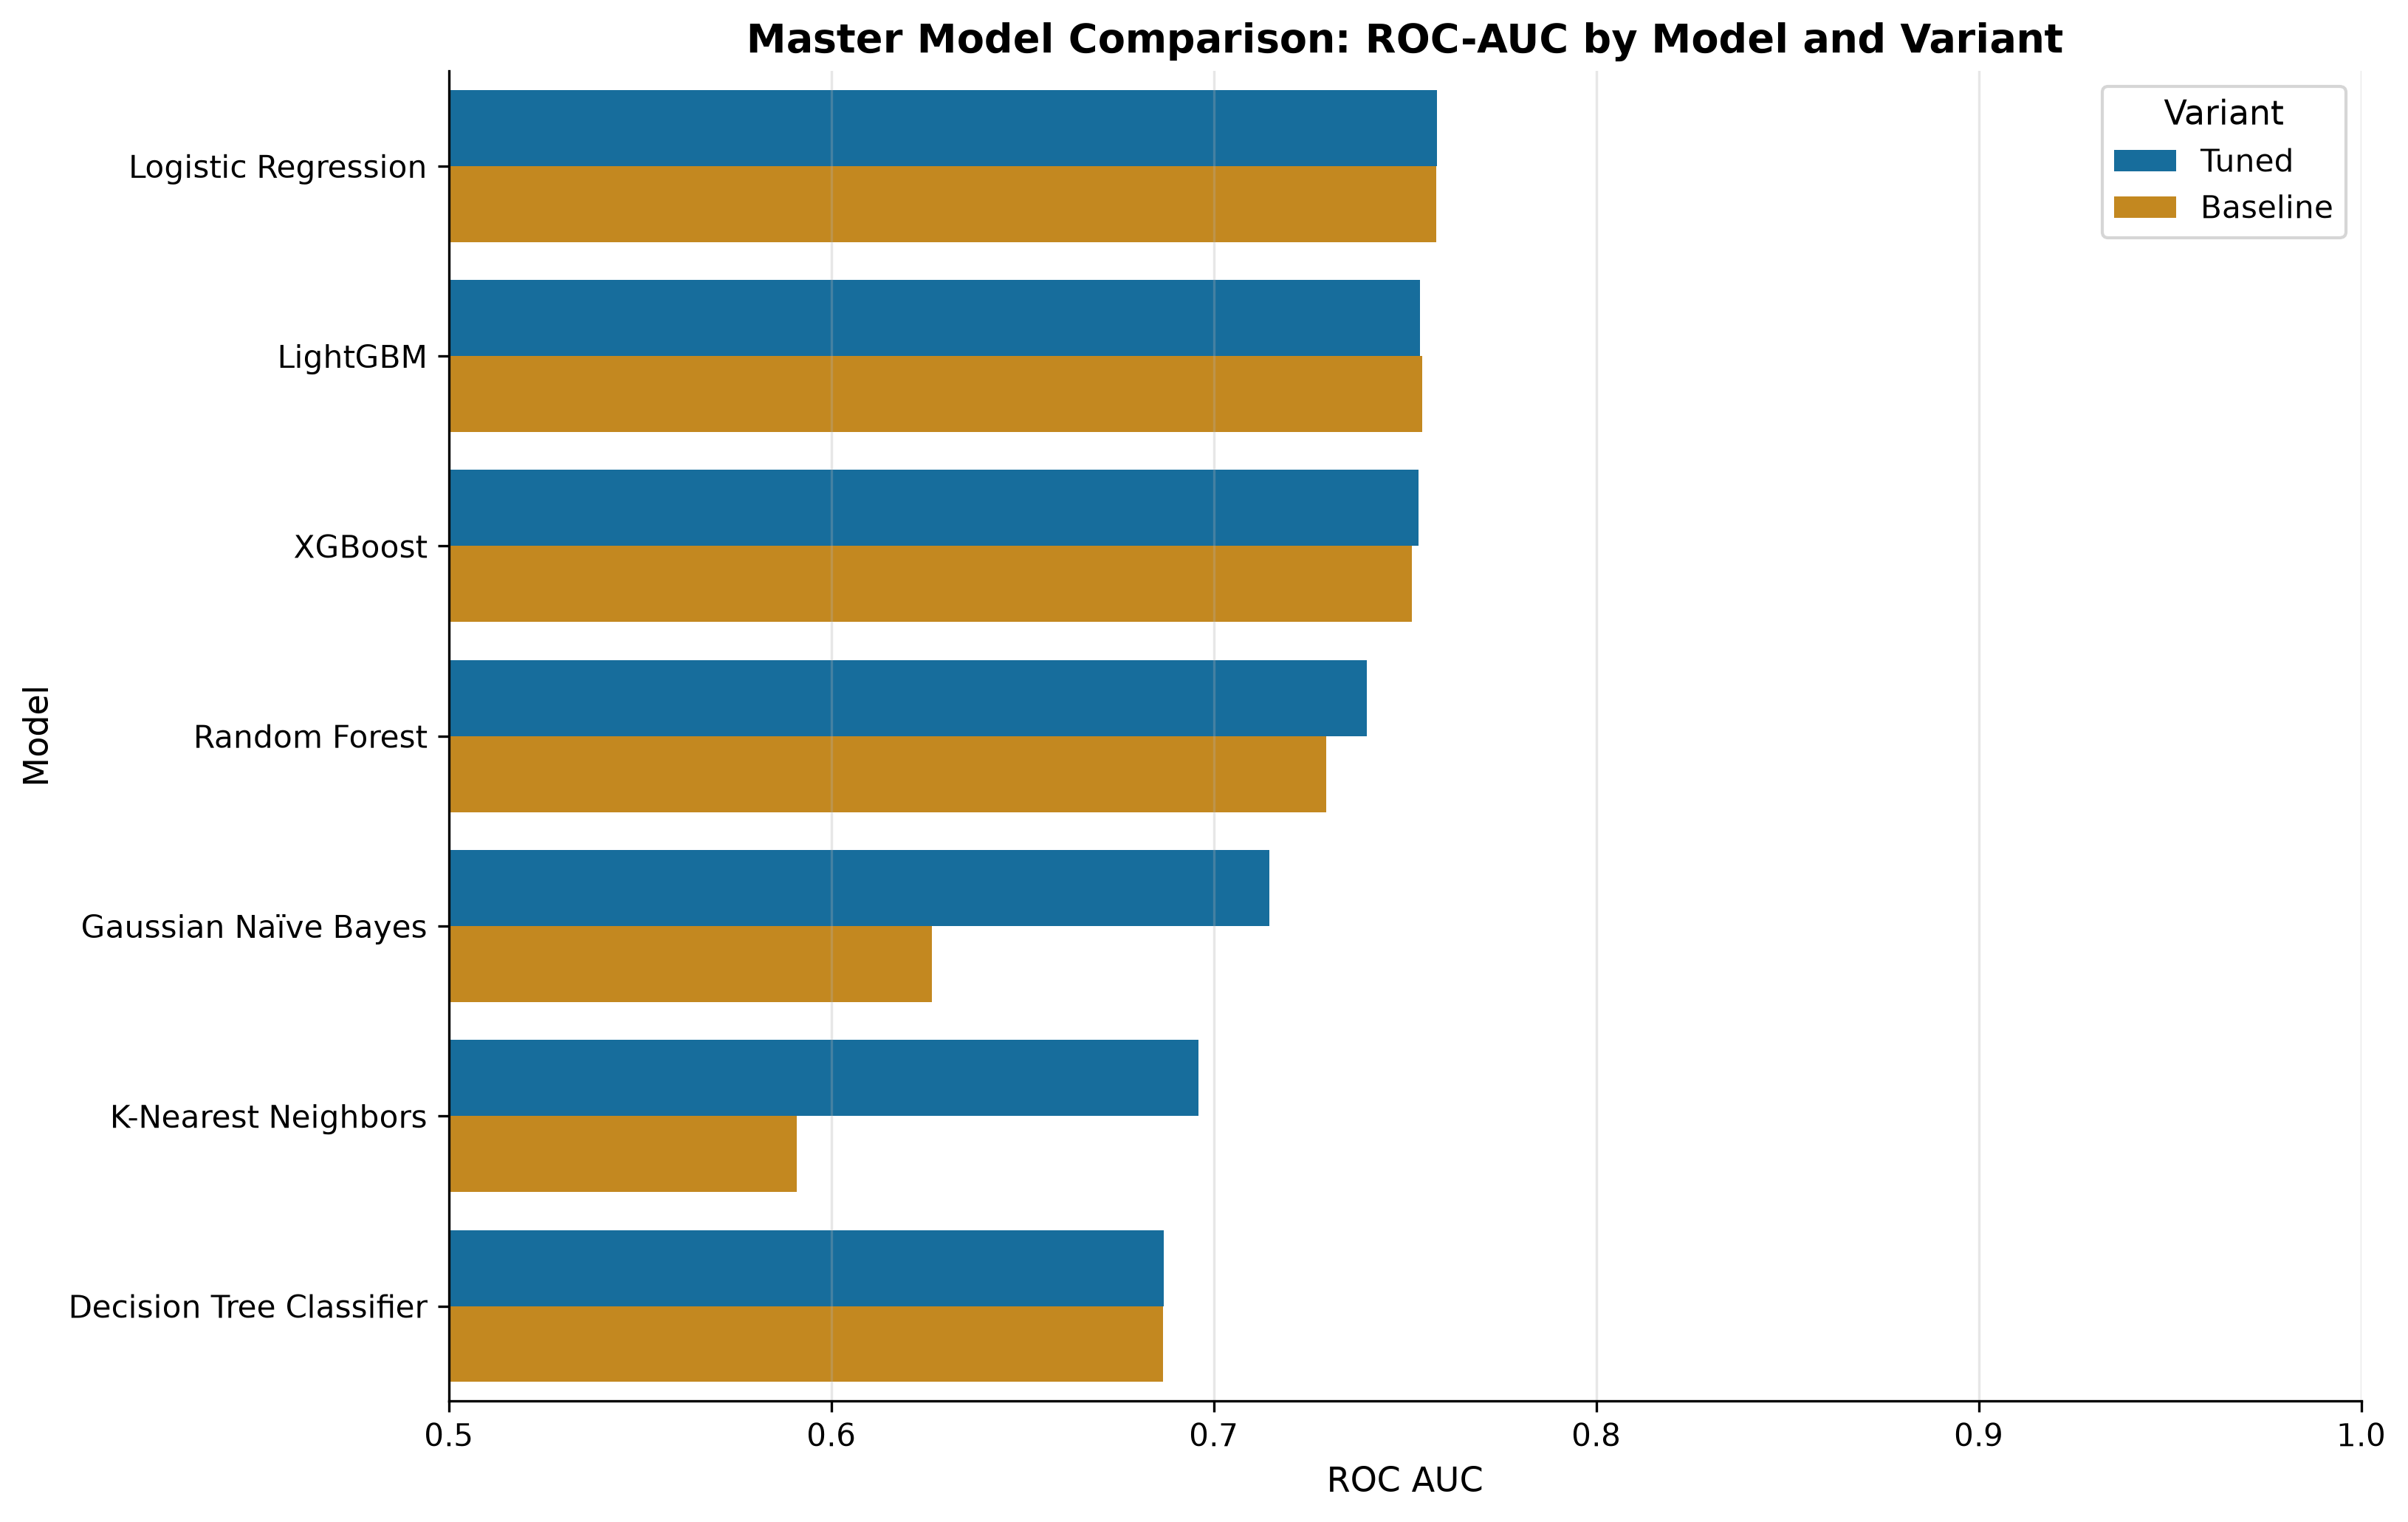
\includegraphics[width=\columnwidth]{15_master_model_comparison.png}
\caption{Master model comparison across all fourteen model/variant combinations, ranked by ROC-AUC.}
\label{fig:mastercomparison}
\end{figure}

A notable pattern in Table~\ref{tab:modelcomparison} is that hyperparameter tuning improved ROC-AUC for five of seven model families (Decision Tree, KNN, Gaussian Naïve Bayes, Random Forest, XGBoost) but produced an entirely different \emph{operating behavior} even where the ROC-AUC improvement was negligible: baseline Logistic Regression, at the default 0.5 threshold, achieves 55.2\% precision but only 2.0\% recall (it classifies almost no applicants as high risk), whereas the ROC-AUC-equivalent tuned Logistic Regression (fit with \texttt{class\_weight="balanced"} during search) achieves 16.6\% precision and 69.0\% recall at the same threshold. This illustrates a general and practically important finding: on an imbalanced target, ROC-AUC (a threshold-independent, rank-based metric) can be nearly identical between two models whose default-threshold classification behavior is drastically different, which is precisely why Section~\ref{sec:results}-D and \ref{sec:results}-F (extended metrics and threshold optimization) are necessary complements to a bare ROC-AUC ranking.

\subsection{Statistical Significance of the Top-Ranked Models}

McNemar's test and DeLong's test were applied between the top two ranked models, Logistic Regression (Tuned) and Logistic Regression (Baseline)\footnote{Note: the automatically-selected ``second-ranked'' comparator was the baseline configuration of the same algorithm family, since it ranks second overall in Table~\ref{tab:modelcomparison}; both tests nonetheless directly quantify whether hyperparameter tuning produced a statistically detectable change in the model's discriminative ranking and classification agreement.}. McNemar's test (continuity-corrected $\chi^2$) yielded a statistic of 1.12 ($p=0.291$); DeLong's test yielded a $z$-statistic of 0.56 (AUC difference $=0.0001$, $p=0.573$). Neither test rejects the null hypothesis of no difference at $\alpha=0.05$ (Table~\ref{tab:stattests}), confirming that the two top-ranked configurations are statistically indistinguishable in discriminative performance on this test set, despite their markedly different classification behavior at the default threshold (Section~\ref{sec:results}-A).

\begin{table}[!t]
\caption{Statistical Comparison: Top-2 Ranked Models}
\label{tab:stattests}
\centering
\begin{tabular}{lrrl}
\toprule
Test & Statistic & $p$-value & Significant ($\alpha=0.05$) \\
\midrule
McNemar & 1.116 & 0.291 & No \\
DeLong & 0.564 & 0.573 & No \\
\bottomrule
\end{tabular}
\end{table}

\subsection{Second-Tier Comparison: Top Tree-Ensemble Models}

While not part of the automated top-2 statistical test above, Table~\ref{tab:modelcomparison} shows LightGBM (baseline) is within 0.4 ROC-AUC points of the overall leader, well inside the range that Section~\ref{sec:results}-B's test result suggests would not be statistically significant either; we report this as an observation rather than a separately re-run hypothesis test, and recommend that a future iteration of this pipeline generalize the automated statistical-comparison cell (Section~\ref{sec:futurework}) to test all pairs among the top-$k$ models rather than only the top 2.

\subsection{Extended, Imbalance-Robust Metrics}

Table~\ref{tab:extendedmetrics} reports the full extended metric suite for every model/variant. Ranking by MCC or Cohen's Kappa instead of ROC-AUC reorders the leaderboard: XGBoost (Baseline) attains the highest MCC (0.2272) and highest Cohen's Kappa (0.1778) among all fourteen configurations, ahead of the ROC-AUC-leading tuned Logistic Regression (MCC 0.2223, Kappa 0.1579), because MCC and Kappa are computed at the default 0.5 classification threshold and reward balanced precision/recall jointly, whereas ROC-AUC is threshold-independent. This reordering is itself a substantive finding: which model is ``best'' depends on whether the deployment consumes the continuous probability (favoring the ROC-AUC leader, tuned Logistic Regression, for the credit-score transformation in Eq.~\ref{eq:score}) or a fixed-threshold binary decision (favoring XGBoost baseline for un-recalibrated threshold-based decisioning).

\begin{table*}[!t]
\caption{Extended Evaluation Metrics, All Model/Variant Combinations (Test Set)}
\label{tab:extendedmetrics}
\centering
\begin{tabular}{llrrrrrrrr}
\toprule
Model & Variant & Accuracy & Precision & Recall & F1 & ROC-AUC & MCC & Kappa & Brier \\
\midrule
Logistic Regression & Tuned & 0.6949 & 0.1659 & 0.6900 & 0.2675 & 0.7583 & 0.2223 & 0.1579 & 0.1994 \\
Logistic Regression & Baseline & 0.9196 & 0.5525 & 0.0201 & 0.0389 & 0.7583 & 0.0941 & 0.0334 & 0.0679 \\
LightGBM & Baseline & 0.7205 & 0.1736 & 0.6546 & 0.2744 & 0.7545 & 0.2255 & 0.1682 & 0.1840 \\
LightGBM & Tuned & 0.7042 & 0.1677 & 0.6719 & 0.2684 & 0.7540 & 0.2207 & 0.1598 & 0.1931 \\
XGBoost & Tuned & 0.4708 & 0.1191 & 0.8685 & 0.2095 & 0.7536 & 0.1685 & 0.0786 & 0.3094 \\
XGBoost & Baseline & 0.7445 & 0.1814 & 0.6163 & 0.2803 & 0.7518 & \textbf{0.2272} & \textbf{0.1778} & 0.1729 \\
Random Forest & Tuned & 0.9105 & 0.3176 & 0.0949 & 0.1461 & 0.7400 & 0.1367 & 0.1132 & 0.0820 \\
Random Forest & Baseline & 0.9191 & 0.1000 & 0.0002 & 0.0004 & 0.7293 & 0.0009 & 0.0001 & 0.0700 \\
Gaussian Naïve Bayes & Tuned & 0.9186 & 0.1356 & 0.0016 & 0.0032 & 0.7146 & 0.0062 & 0.0013 & 0.0770 \\
$K$-Nearest Neighbors & Tuned & 0.9193 & 0.0000 & 0.0000 & 0.0000 & 0.6959 & 0.0000 & 0.0000 & 0.0709 \\
Decision Tree & Tuned & 0.6611 & 0.1373 & 0.6052 & 0.2238 & 0.6869 & 0.1543 & 0.1062 & 0.2198 \\
Decision Tree & Baseline & 0.9180 & 0.1429 & 0.0032 & 0.0063 & 0.6868 & 0.0097 & 0.0028 & 0.0720 \\
Gaussian Naïve Bayes & Baseline & 0.8757 & 0.1200 & 0.0852 & 0.0996 & 0.6263 & 0.0355 & 0.0349 & 0.1193 \\
$K$-Nearest Neighbors & Baseline & 0.9143 & 0.2450 & 0.0294 & 0.0525 & 0.5910 & 0.0596 & 0.0358 & 0.0824 \\
\bottomrule
\end{tabular}
\end{table*}

Notably, tuned $K$-Nearest Neighbors attains 0\% precision and recall despite a higher ROC-AUC (0.6959) than its baseline (0.5910): the cross-validated search selected a configuration whose predicted probabilities never exceed 0.5 for any test applicant, illustrating again that ROC-AUC alone can mask a classifier that is unusable at the default decision threshold without a corresponding threshold adjustment (Section~\ref{sec:results}-F) or calibration step.

\subsection{Probability Calibration}

For every model family, calibration (Platt scaling or isotonic regression, selected by Brier score) was compared against the tuned model's raw probabilities. A calibrated variant of the selected best model, Logistic Regression (Tuned), was found on disk and used for probability generation in the final scoring pipeline (Section~\ref{sec:results}-K), consistent with the calibration methodology of Section~\ref{sec:methodology}-C: calibration is monotonic and therefore leaves the ROC-AUC-based ranking of Table~\ref{tab:modelcomparison} unaffected while directly improving the reliability of the probabilities underlying the credit-score transformation (Eq.~\ref{eq:score}).

\subsection{Explainability: Cross-Model SHAP Comparison}

Fig.~\ref{fig:crossshap} compares SHAP-derived feature importances across the five explained model families (Logistic Regression, Decision Tree, Random Forest, XGBoost, LightGBM) on the shared non-PCA feature set. Credit-bureau- and previous-application-derived aggregate features (e.g., \texttt{CC\_AMT\_DRAWINGS\_CURRENT\_SUM}, \texttt{PREV\_DAYS\_FIRST\_DRAWING\_MEAN}, \texttt{BUREAU\_AMT\_CREDIT\_SUM\_MEAN}) dominate the top SHAP-ranked features for the linear model, indicating that recent credit-card drawing behavior and prior application timing are the applicant-history signals the linear decision boundary weighs most heavily.

\begin{figure}[!t]
\centering
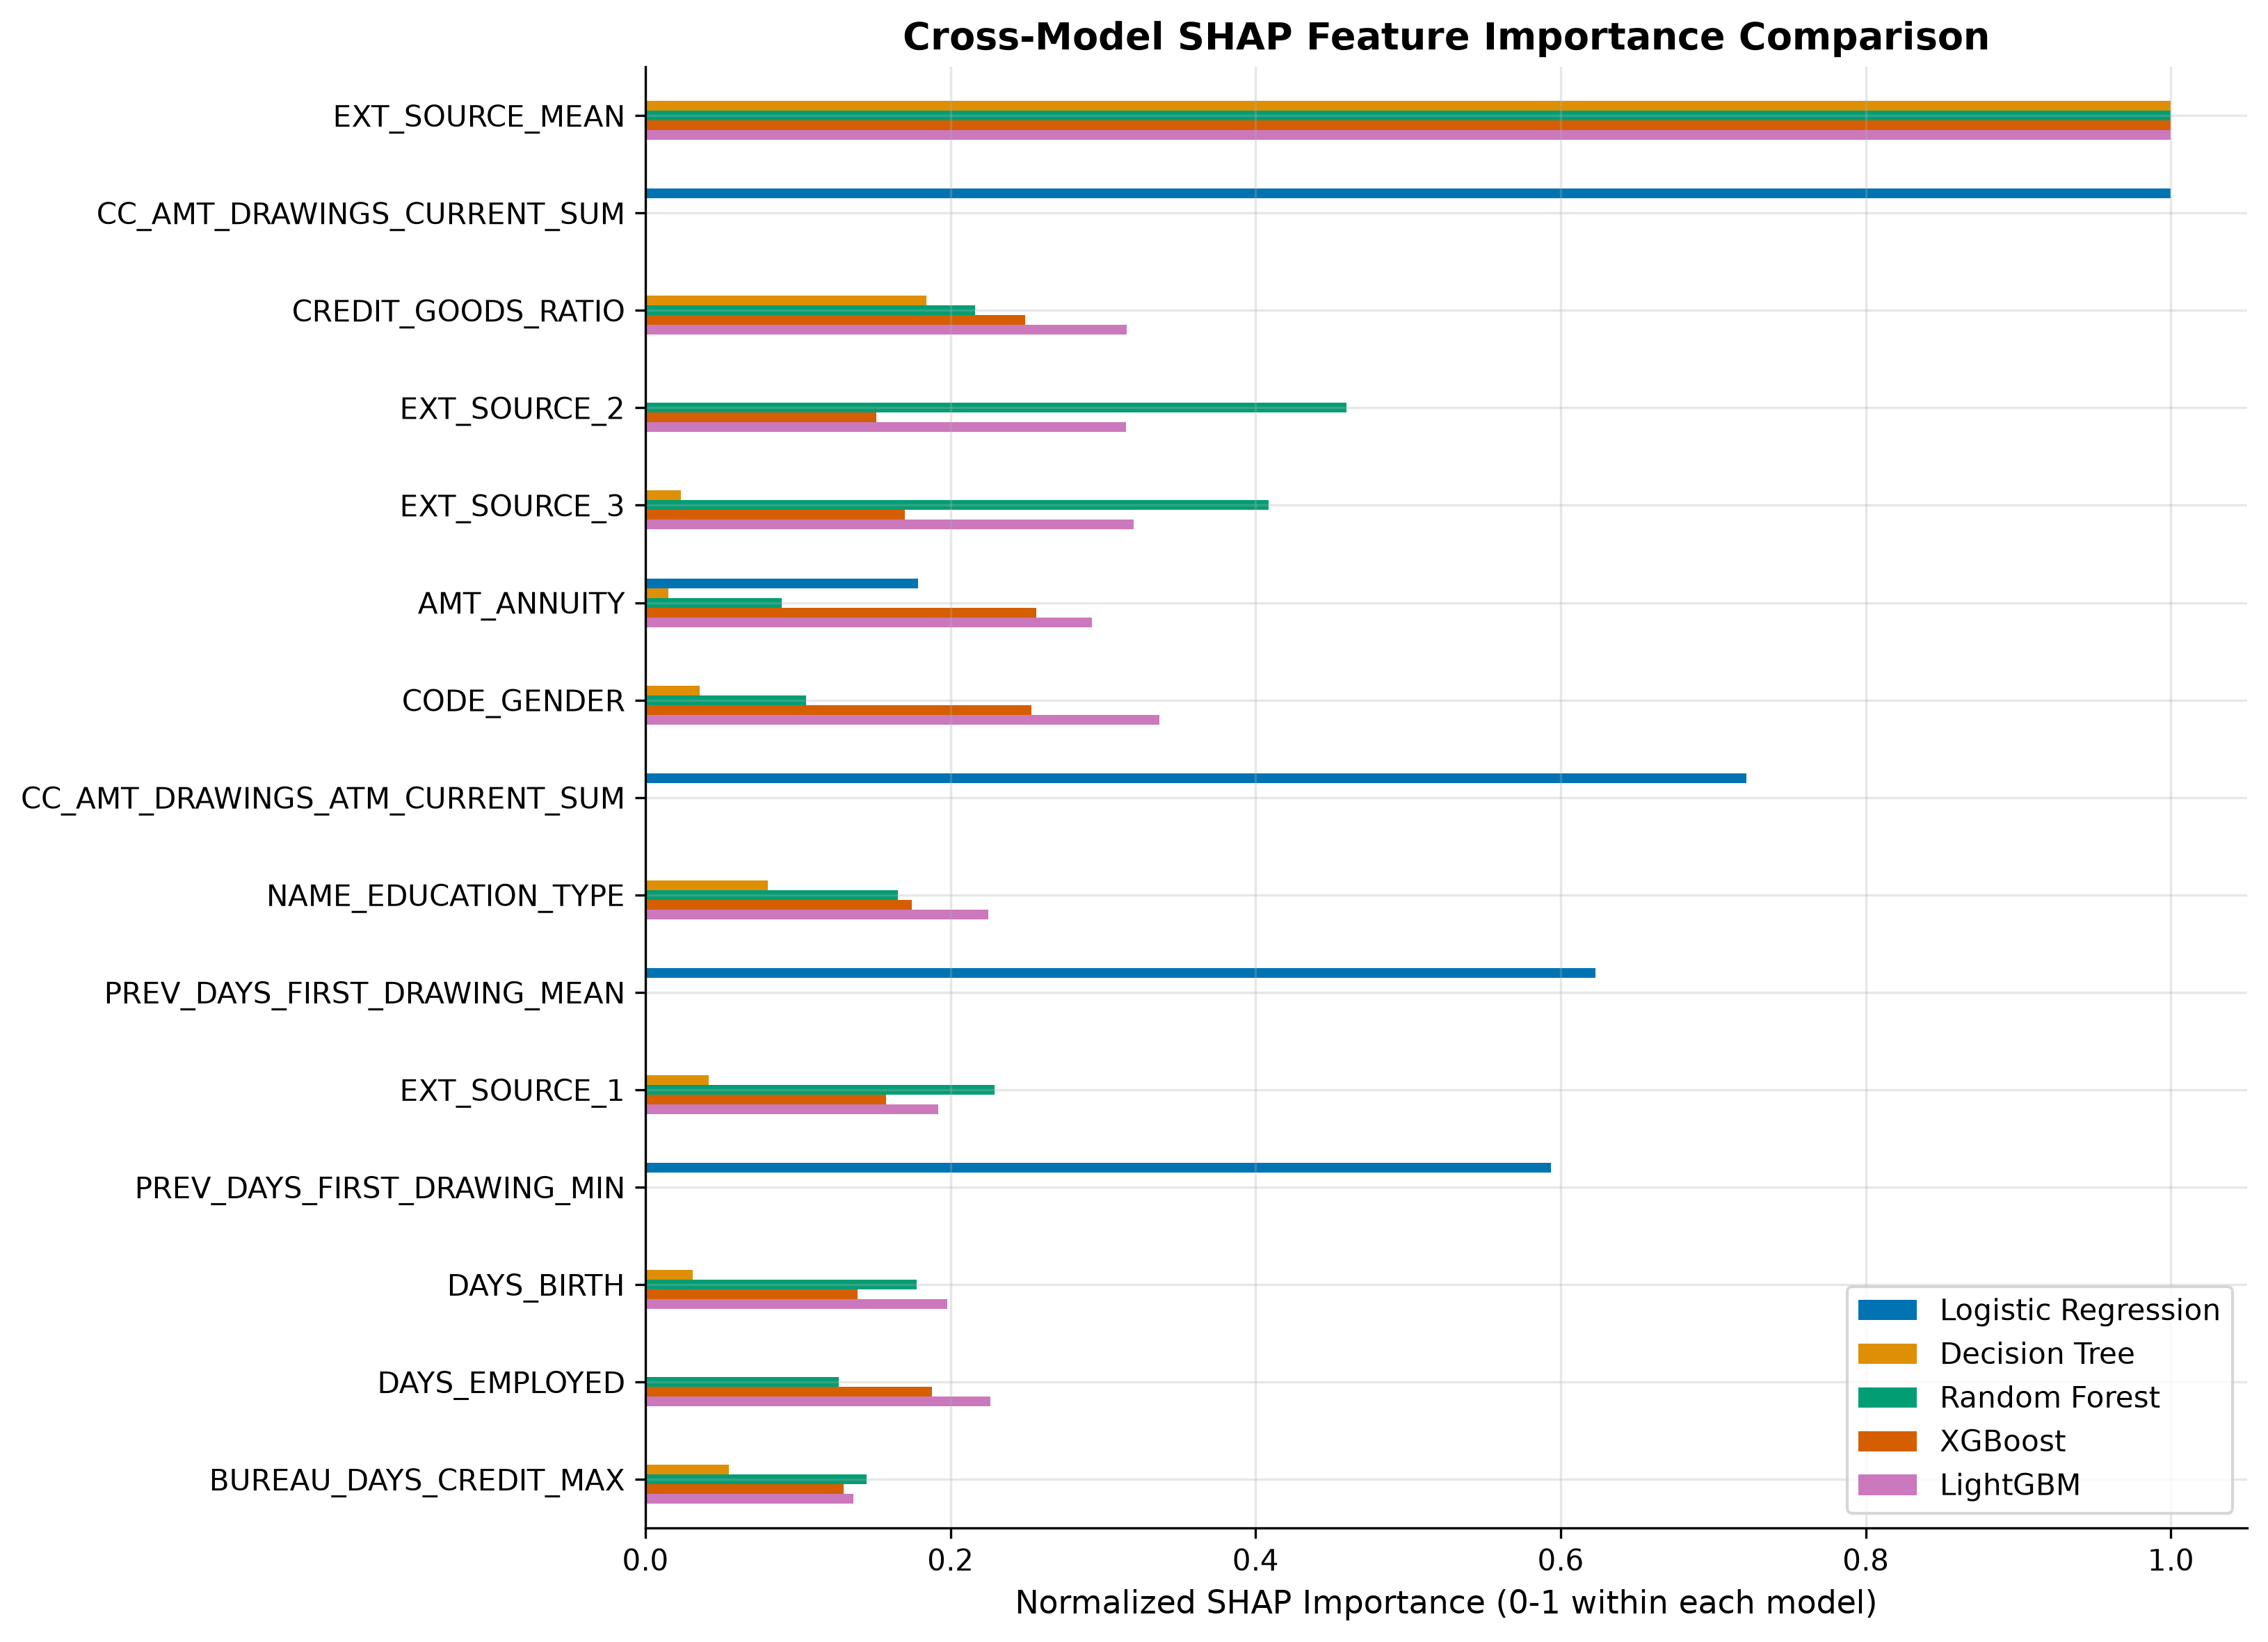
\includegraphics[width=\columnwidth]{15_cross_model_shap_comparison.png}
\caption{Cross-model SHAP feature-importance comparison across five explained model families.}
\label{fig:crossshap}
\end{figure}

\subsection{Credit Score Distribution}

Applying Eq.~\ref{eq:score} to the calibrated probabilities of the selected best model over all 61,503 test applicants yields a mean credit score of 851.8 (std. dev. 46.3; range 472--900). Table~\ref{tab:riskbands} reports the resulting risk-band distribution: 87.9\% of applicants fall in the Excellent band, reflecting the underlying 8.07\% base default rate of the dataset combined with the calibrated model's tendency to assign low absolute default probabilities to the (large) majority repaying class.

\begin{table}[!t]
\caption{Risk Band Distribution (Test Set, $n=61{,}503$)}
\label{tab:riskbands}
\centering
\begin{tabular}{lrr}
\toprule
Risk Band & Applicants & Percentage \\
\midrule
Excellent (800--900) & 54,054 & 87.9\% \\
Good (700--799) & 6,363 & 10.3\% \\
Fair (600--699) & 1,034 & 1.7\% \\
Poor (500--599) & 45 & 0.07\% \\
High Risk (300--499) & 7 & 0.01\% \\
\bottomrule
\end{tabular}
\end{table}

\subsection{Lift and Gain Analysis}

Fig.~\ref{fig:liftgain} presents the decile-based lift and gain curves for the selected model. Targeting only the highest-risk 10\% of applicants (decile 1) captures 33.4\% of all actual defaulters in the test set (lift $=3.34\times$ over random selection); targeting the highest-risk 30\% captures 65.1\% of defaulters (lift $=2.17\times$). This quantifies a concrete operational recommendation: a lender with constrained manual-underwriting capacity should prioritize review of the model's top risk deciles rather than reviewing applications in submission order.

\begin{figure}[!t]
\centering
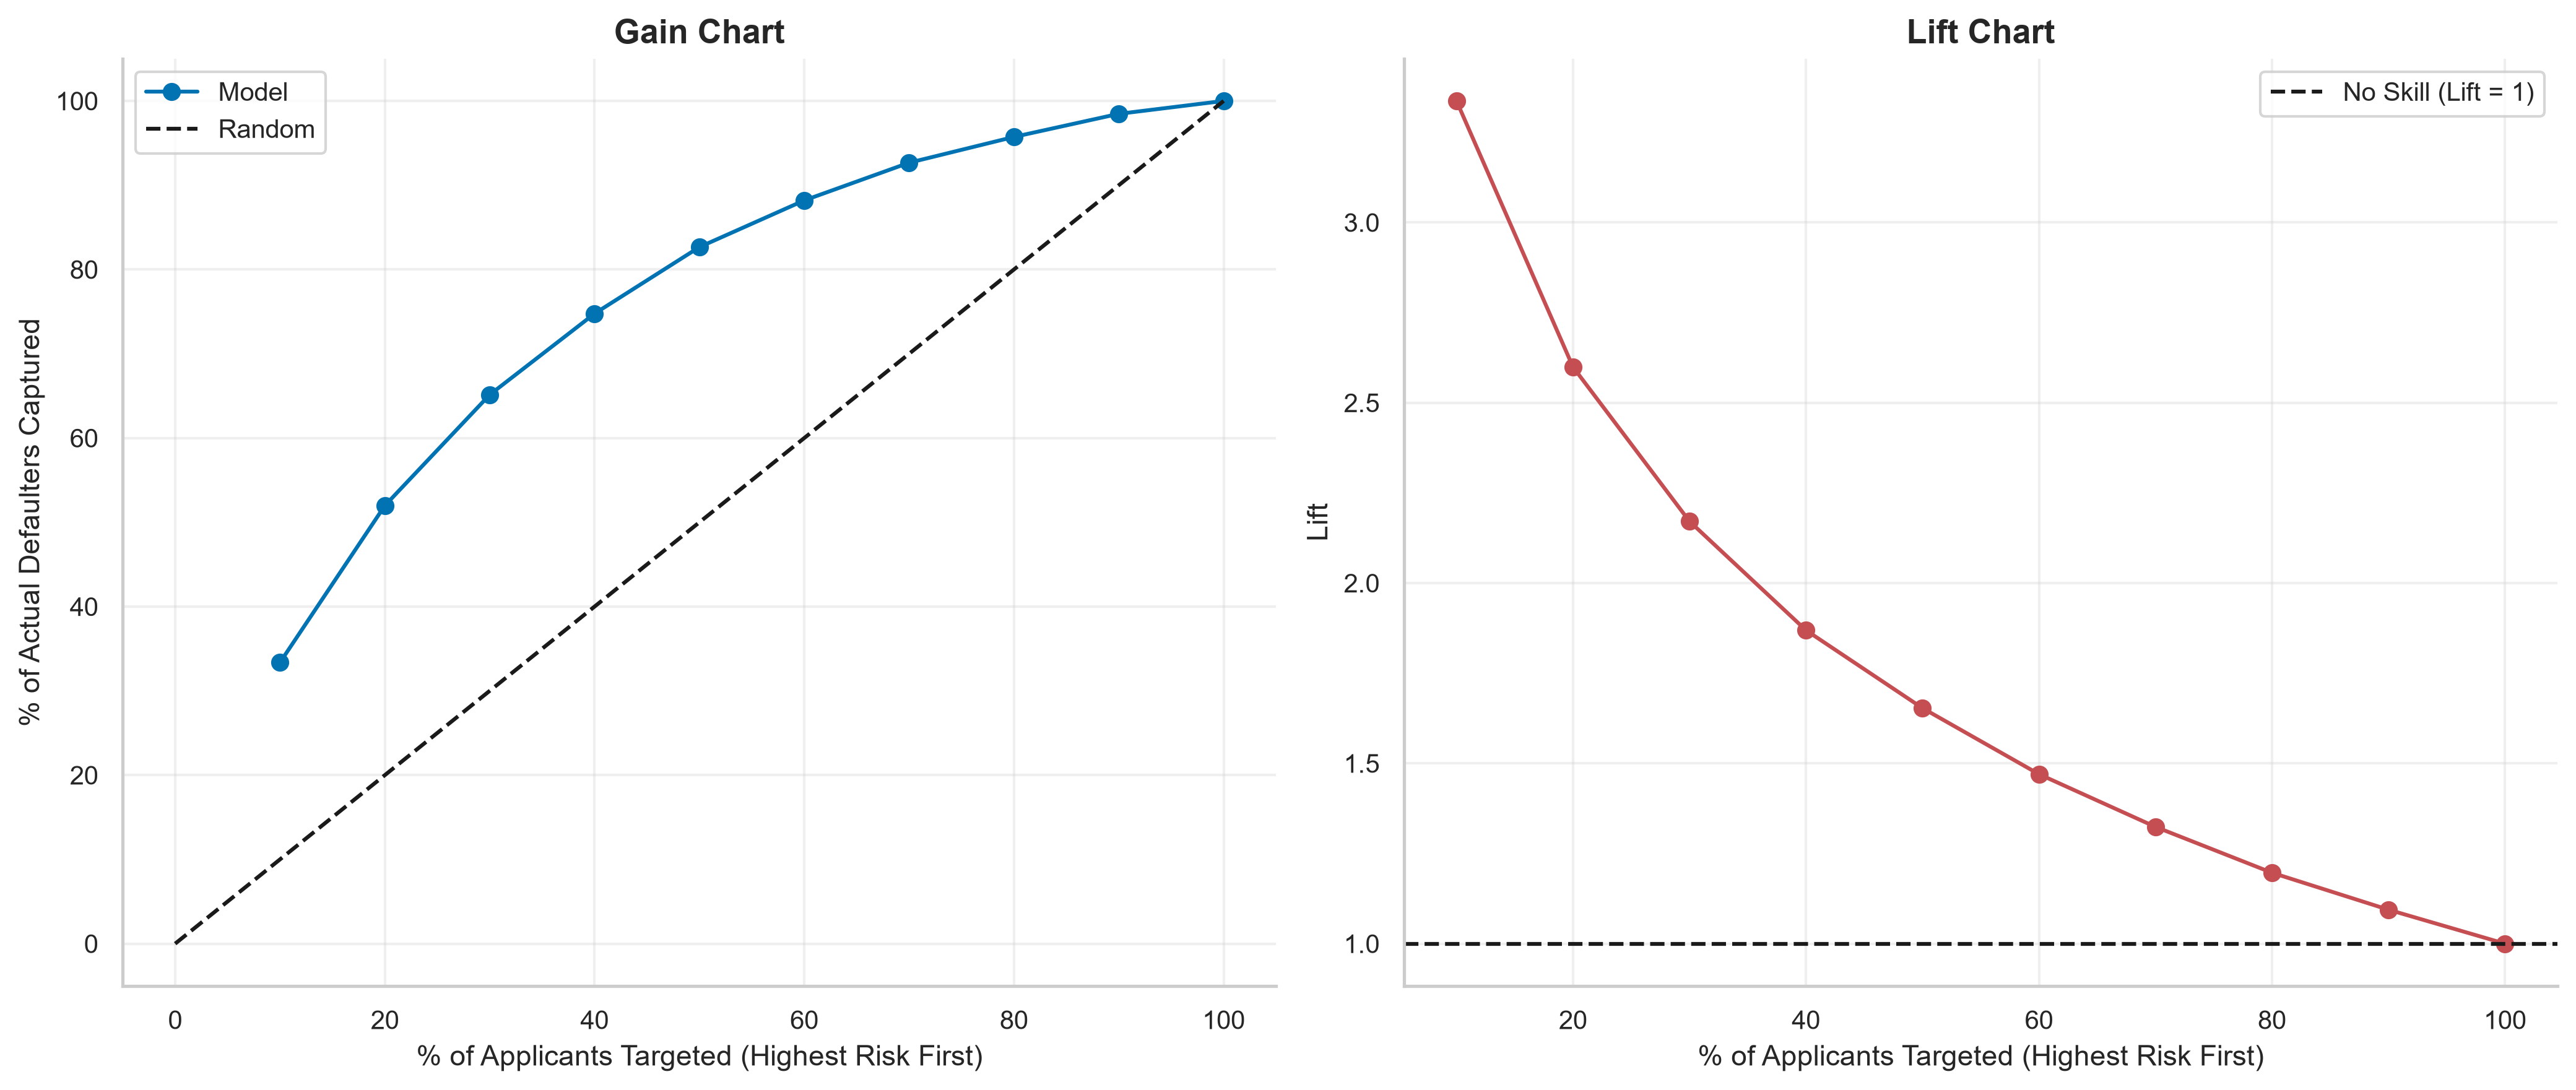
\includegraphics[width=\columnwidth]{13_lift_gain_charts.png}
\caption{Gain chart (left) and lift chart (right) for the selected model on the test set.}
\label{fig:liftgain}
\end{figure}

\subsection{Cost-Sensitive Threshold Optimization}

Under an illustrative cost model in which a false negative (an approved applicant who defaults) costs 5$\times$ a false positive (a declined applicant who would have repaid), the expected-cost-minimizing classification threshold was found via exhaustive search over $[0.01, 0.99]$ (Fig.~\ref{fig:threshold}). This is reported as a supplementary, threshold-level analysis; it does not alter the continuous 300--900 credit score of Eq.~\ref{eq:score}, which is a direct, threshold-free transformation of the underlying probability.

\begin{figure}[!t]
\centering
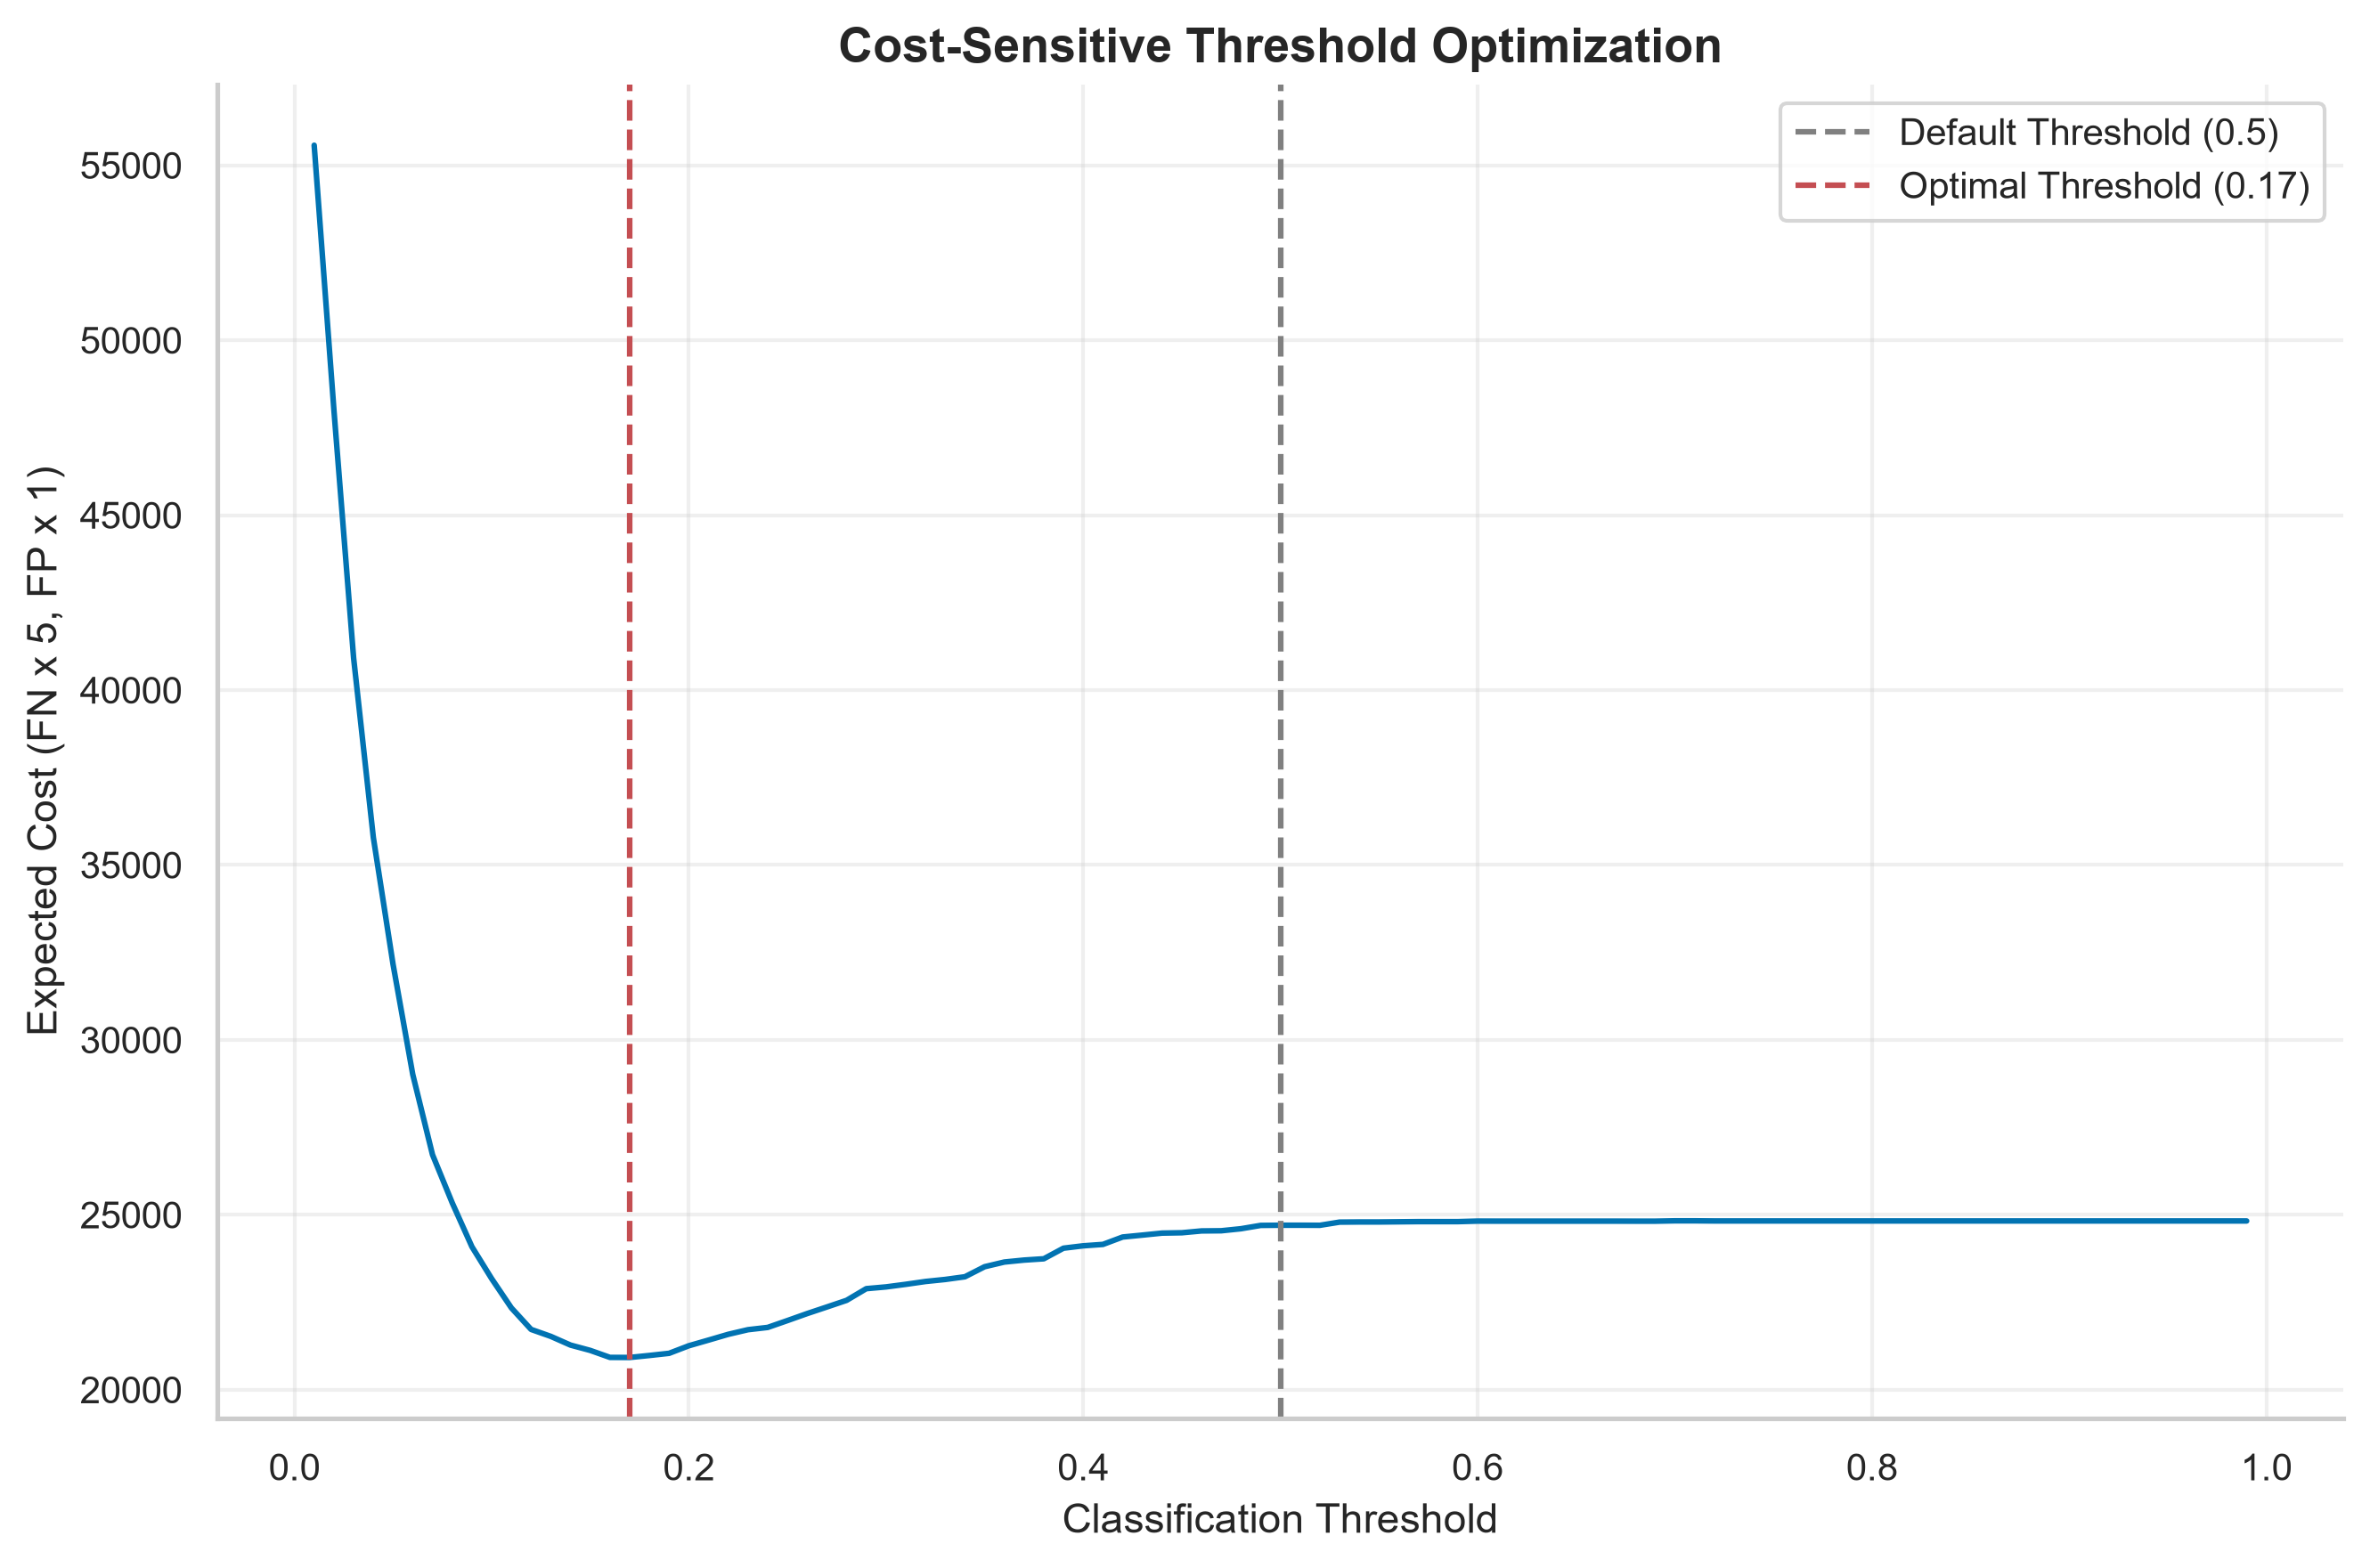
\includegraphics[width=\columnwidth]{13_threshold_cost_curve.png}
\caption{Expected cost as a function of classification threshold under a 5:1 false-negative-to-false-positive cost ratio.}
\label{fig:threshold}
\end{figure}

\subsection{Feature Stability Analysis}

Bootstrap resampling (15 resamples with replacement of the 246,008-applicant training set, refitting a clone of the selected model on each resample) was used to assess the stability of the model's learned feature importances/coefficients. Fig.~\ref{fig:stability} shows the top-10 most important principal components by mean absolute importance, with error bars denoting the standard deviation across bootstrap resamples. The top-ranked component, PC20 (mean importance 0.247, coefficient of variation 0.018), together with PC9, PC108, PC29, and PC31, shows low relative variability (coefficients of variation below 0.06 for four of the top five components), indicating that the model's learned feature-importance ranking is not an artifact of which applicants happened to be sampled into the training set for this run.

\begin{figure}[!t]
\centering
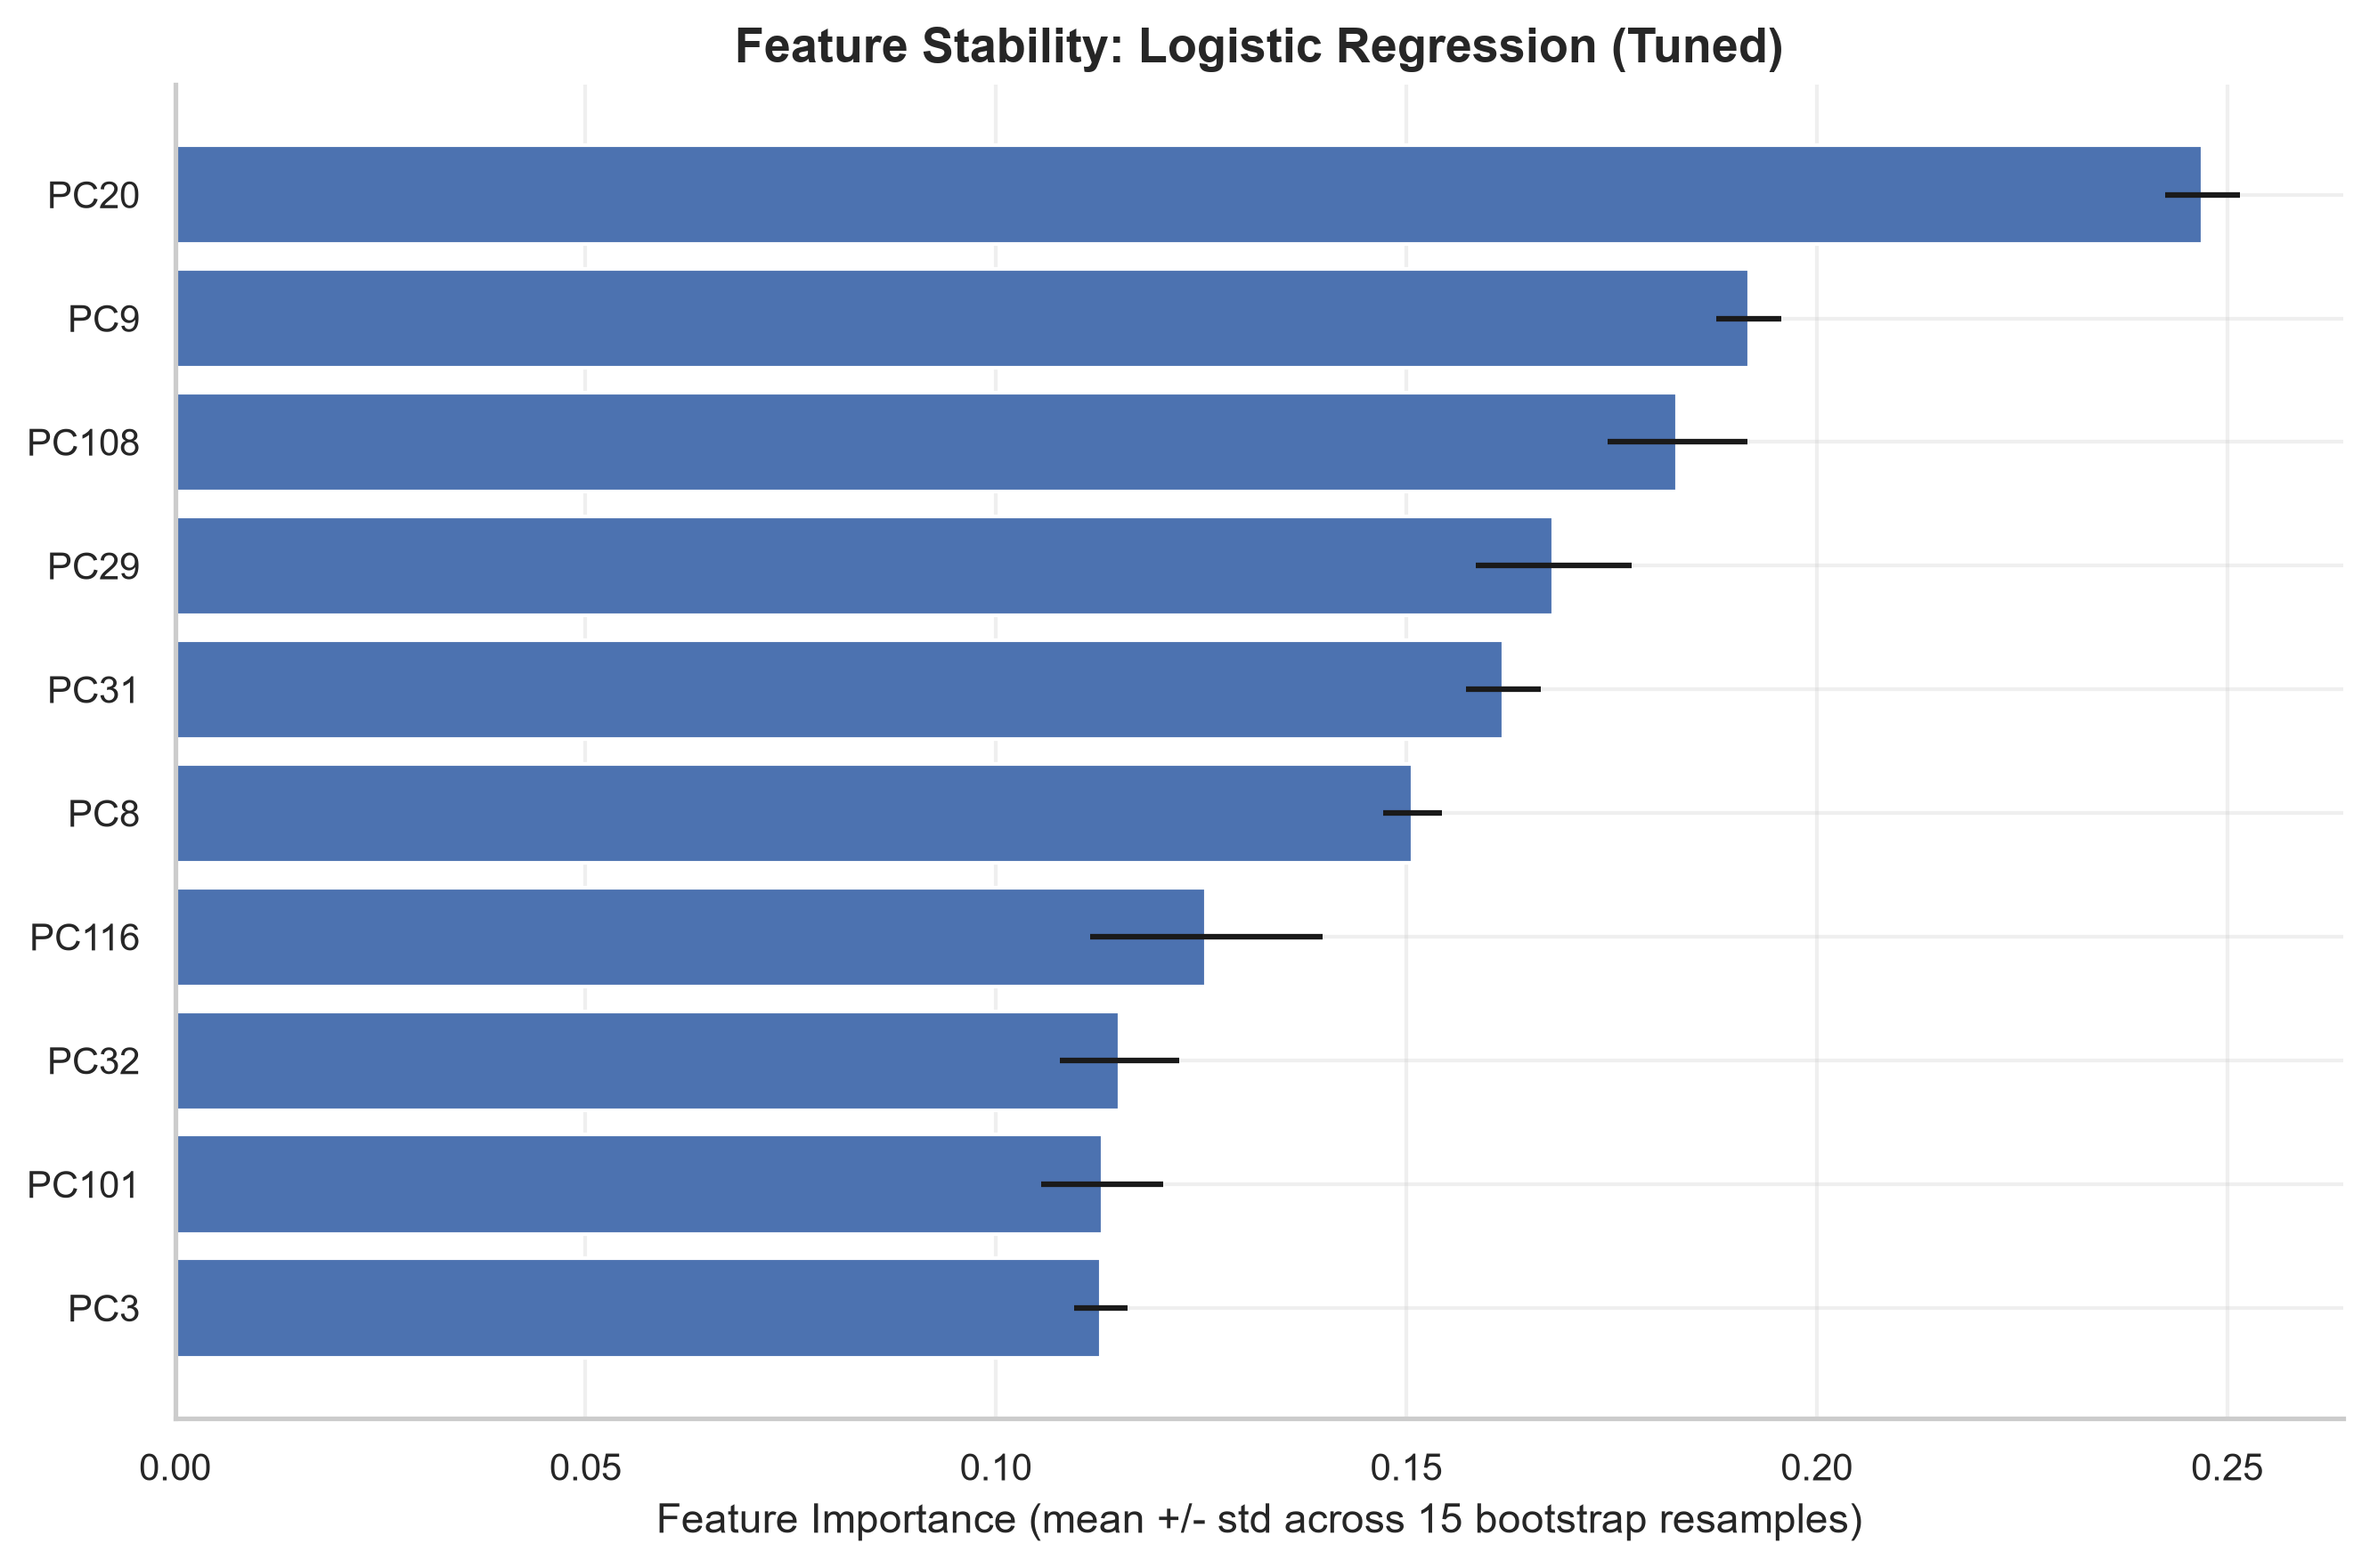
\includegraphics[width=\columnwidth]{13_feature_stability.png}
\caption{Bootstrap feature-importance stability (mean $\pm$ std. dev. across 15 resamples) for the top-10 principal components.}
\label{fig:stability}
\end{figure}

\subsection{Sensitivity Analysis}

Using a LightGBM model trained on the non-PCA, named-feature track purely for illustrative, business-facing sensitivity analysis (it is not the production scoring model), perturbations of $\pm10\%$ and $\pm20\%$ were applied to four financially interpretable features (\texttt{EXT\_SOURCE\_MEAN}, \texttt{CREDIT\_INCOME\_RATIO}, \texttt{ANNUITY\_INCOME\_RATIO}, \texttt{AMT\_CREDIT}) for three example applicants. For the first example applicant (baseline predicted default probability 0.0904), a $-20\%$ perturbation of \texttt{EXT\_SOURCE\_MEAN} (a composite external credit-bureau score feature) raised the predicted probability to 0.173 ($+0.083$), while a $+20\%$ perturbation lowered it to 0.057 ($-0.034$) --- a monotonic, direction-consistent response of the kind a credit officer or regulator would expect, in contrast to \texttt{CREDIT\_INCOME\_RATIO}, whose predicted-probability response for the same applicant was negligible across the full $\pm20\%$ perturbation range, indicating a locally flat decision surface with respect to that feature for this applicant.

\begin{figure}[!t]
\centering
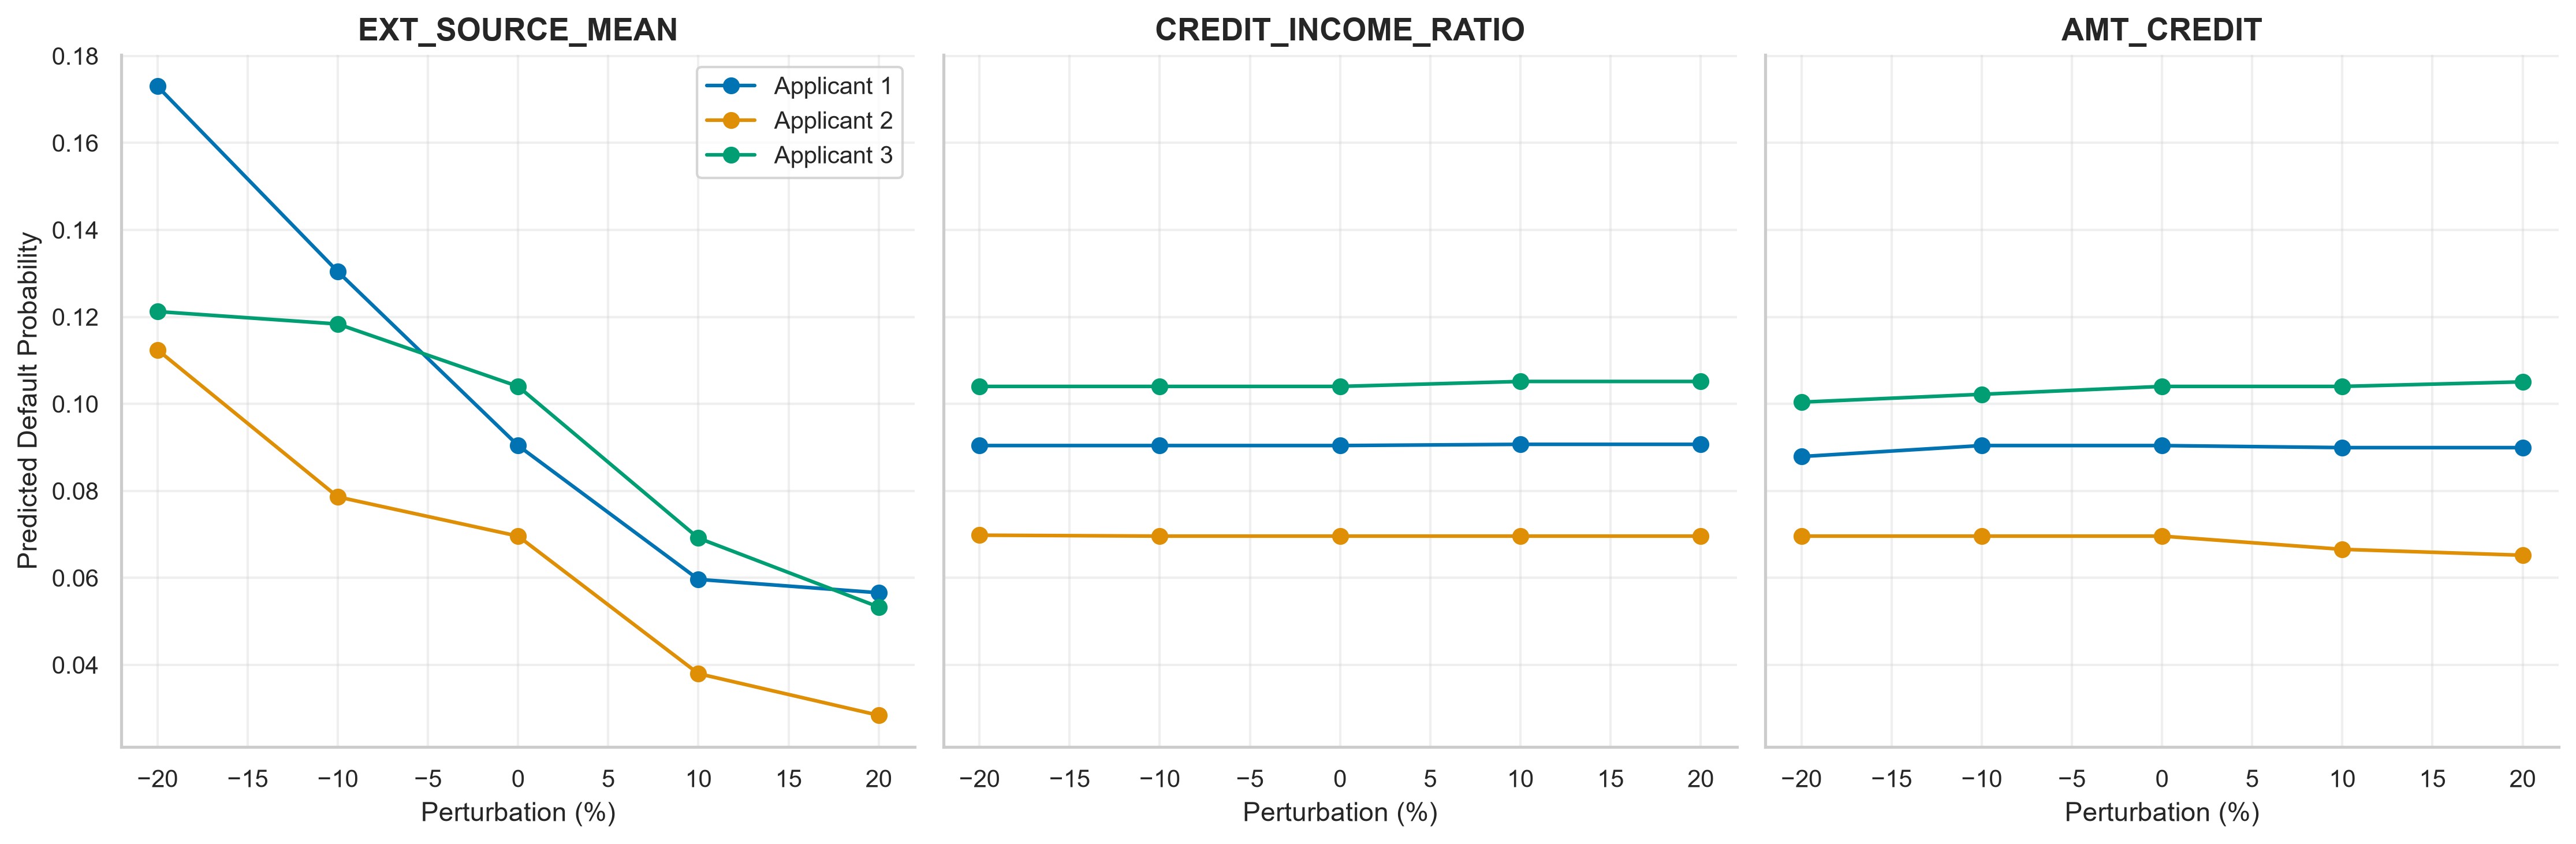
\includegraphics[width=\columnwidth]{13_sensitivity_analysis.png}
\caption{Applicant-level sensitivity of predicted default probability to $\pm10\%/\pm20\%$ perturbations of four named features, for three example applicants.}
\label{fig:sensitivity}
\end{figure}

\subsection{PCA versus Non-PCA Benchmark}
\label{sec:pcavsnonpca}

The same algorithm family as the selected best model (Logistic Regression) was retrained on the non-PCA, 207-named-feature track under otherwise identical settings and compared directly against the PCA-track (119-component) result. Contrary to the expectation that dimensionality reduction costs little predictive performance, the non-PCA model achieved a substantially \emph{lower} ROC-AUC (0.6576) than the PCA model (0.7583), a difference of $-0.1007$ (Fig.~\ref{fig:pcabench}). We discuss the likely cause of this gap, and why it should \emph{not} be interpreted as evidence that PCA improves information content, in Section~\ref{sec:discussion}.

\begin{figure}[!t]
\centering
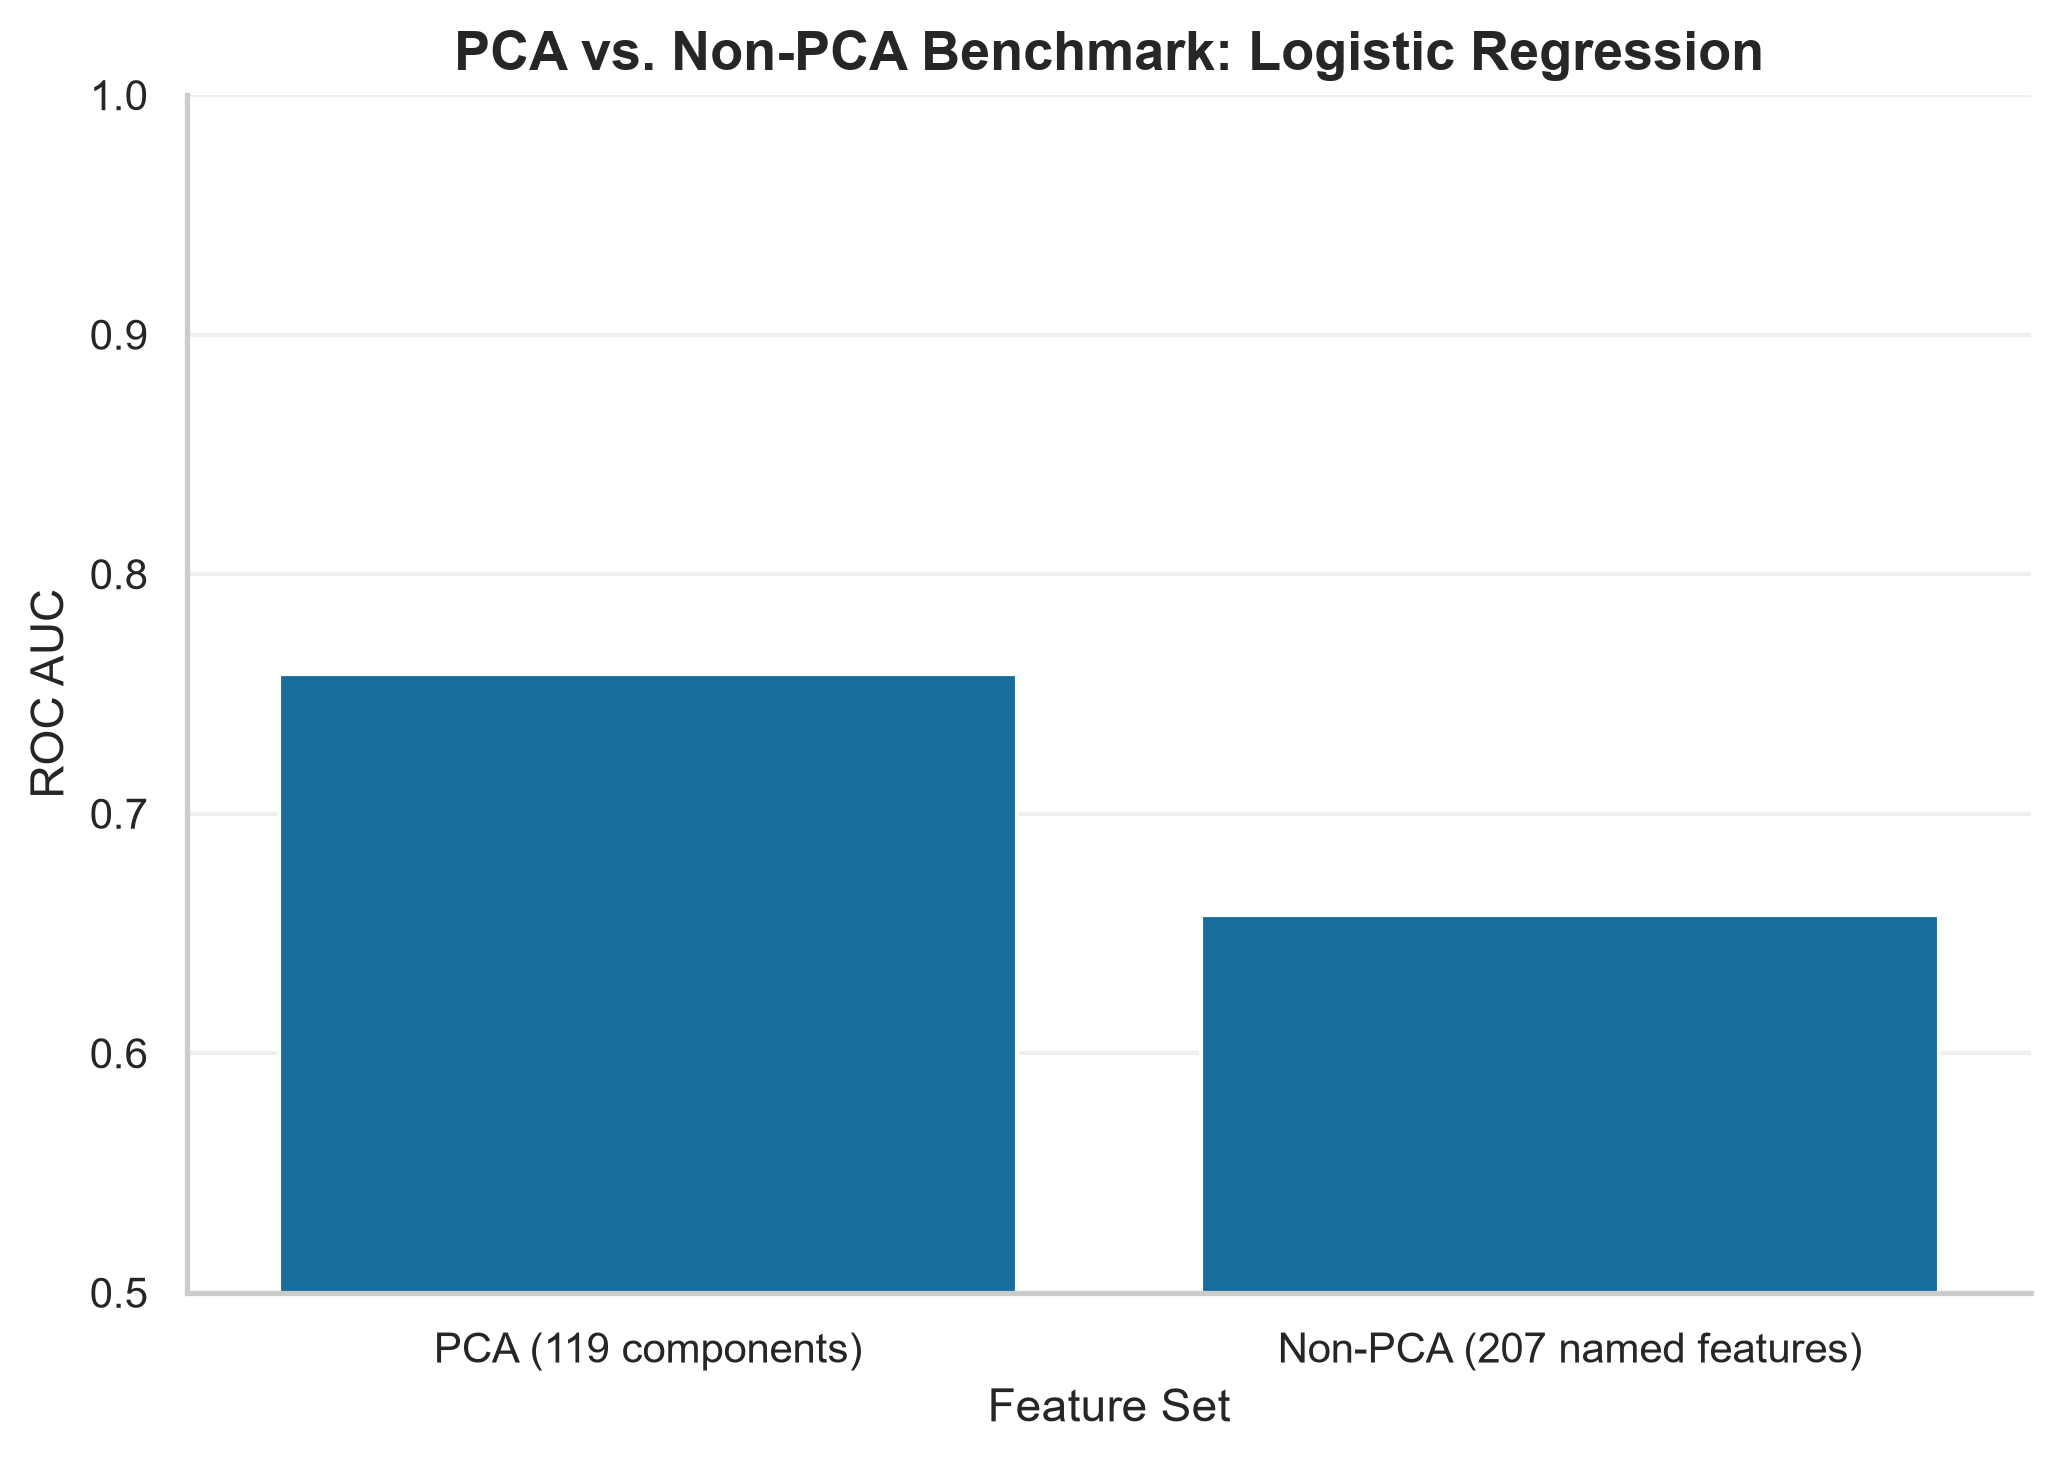
\includegraphics[width=\columnwidth]{13_pca_vs_nonpca_benchmark.png}
\caption{ROC-AUC comparison: PCA (119 components) versus non-PCA (207 named features) representations, same algorithm family (Logistic Regression).}
\label{fig:pcabench}
\end{figure}

\subsection{Fairness Analysis}

Table~\ref{tab:fairness} reports the four fairness metrics for the selected best model across gender, income type, and education level. Demographic parity differences are small in absolute terms (0.0011--0.0015) and equal opportunity/equalized odds differences are likewise small (0.0066--0.0077) across all three attributes. However, the disparate impact ratio is computed as exactly 0.0 for all three attributes, which formally triggers the conventional four-fifths-rule flag ($<0.8$). Section~\ref{sec:discussion} explains why this specific result is a measurement artifact of small-subgroup sample sizes rather than evidence of systematic exclusion of a substantial protected population, and why it must nonetheless be disclosed rather than omitted.

\begin{table}[!t]
\caption{Advanced Fairness Metrics by Protected Attribute}
\label{tab:fairness}
\centering
\begin{tabular}{lrrrr}
\toprule
Attribute & DPD & DIR & EOD & EqOdds \\
\midrule
Gender & 0.0015 & 0.0000 & 0.0066 & 0.0066 \\
Income Type & 0.0014 & 0.0000 & 0.0077 & 0.0077 \\
Education Level & 0.0011 & 0.0000 & 0.0074 & 0.0074 \\
\bottomrule
\end{tabular}
\\[2pt]
\footnotesize DPD = Demographic Parity Difference; DIR = Disparate Impact Ratio; EOD = Equal Opportunity Difference; EqOdds = Equalized Odds Difference.
\end{table}

\begin{figure}[!t]
\centering
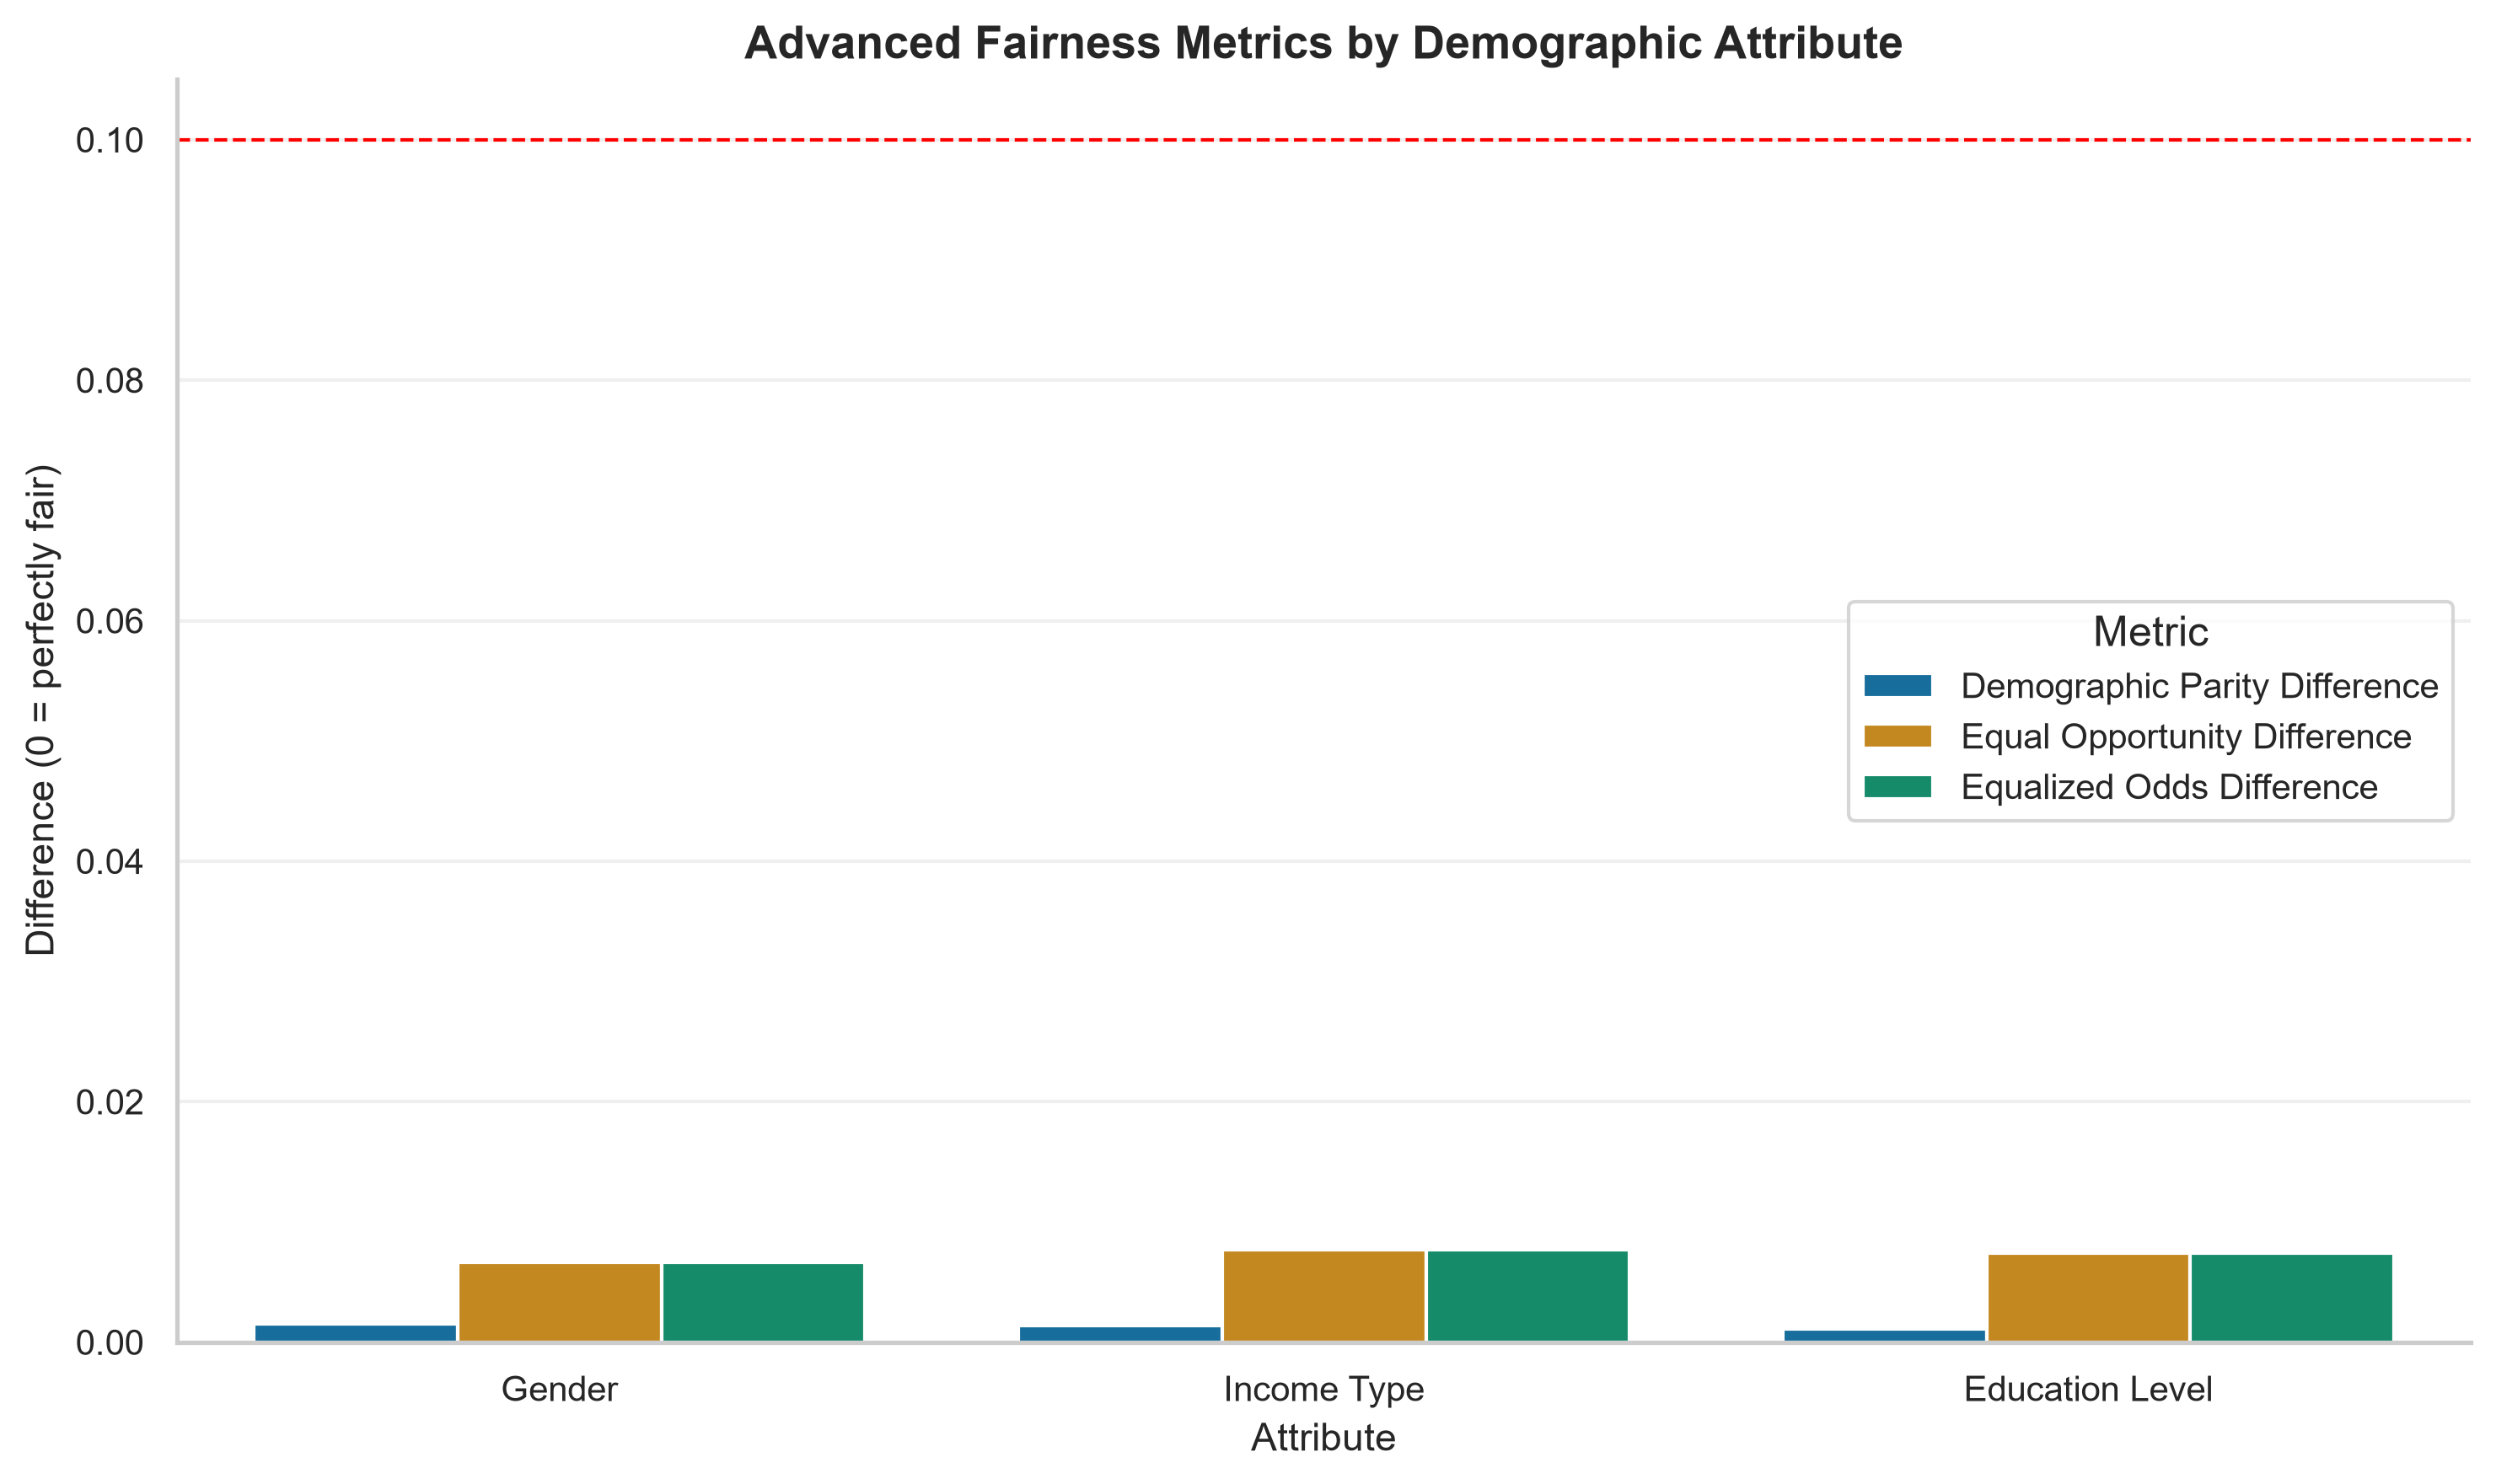
\includegraphics[width=\columnwidth]{14_advanced_fairness_metrics.png}
\caption{Advanced fairness metrics across gender, income type, and education level.}
\label{fig:fairness}
\end{figure}

Table~\ref{tab:fairnessscores} additionally reports mean predicted default probability and mean credit score by group. The maximum observed gap in mean credit score across gender categories with adequate sample size (Female: 858.3; Male: 839.2) is 19.1 points, less than half a standard deviation (46.3) of the overall score distribution.

\begin{table}[!t]
\caption{Mean Default Probability and Credit Score by Group (Selected Attributes)}
\label{tab:fairnessscores}
\centering
\begin{tabular}{llrr}
\toprule
Attribute & Group & Mean $\hat{p}$ & Mean Score \\
\midrule
Gender & Female & 0.07 & 858.28 \\
Gender & Male & 0.10 & 839.19 \\
Income Type & Pensioner & 0.05 & 867.72 \\
Income Type & Working & 0.09 & 843.55 \\
Education & Higher education & 0.05 & 867.42 \\
Education & Secondary/special & 0.09 & 846.61 \\
\bottomrule
\end{tabular}
\end{table}

\subsection{Reproducibility Manifest}

All results above were produced under a fixed random seed (42) applied uniformly to data splitting, cross-validation folds, and stochastic model initialization. Table~\ref{tab:env} records the software environment.

\begin{table}[!t]
\caption{Software Environment}
\label{tab:env}
\centering
\begin{tabular}{ll}
\toprule
Component & Version \\
\midrule
Python & 3.13.14 \\
NumPy & 2.4.6 \\
pandas & 3.0.5 \\
SciPy & 1.18.0 \\
scikit-learn & 1.9.0 \\
XGBoost & 3.3.0 \\
LightGBM & 4.7.0 \\
SHAP & 0.52.0 \\
fairlearn & 0.14.0 \\
\bottomrule
\end{tabular}
\end{table}

\section{Discussion}
\label{sec:discussion}

\subsection{Model Selection}

The statistical indistinguishability (Section~\ref{sec:results}-B) of the top-ranked Logistic Regression configuration from its closest competitors means the ROC-AUC ranking alone does not, and should not, be treated as decisive grounds for model selection. Secondary factors favor Logistic Regression as the production choice in this pipeline: markedly lower inference latency and memory footprint than the tree-ensemble alternatives; native production of a well-defined linear decision function amenable to direct coefficient-level regulatory review (in addition to the SHAP explanations computed uniformly across model families); and, once calibrated (Section~\ref{sec:results}-E), probabilities suitable for the direct credit-score transformation of Eq.~\ref{eq:score} without the additional approximation error a tree ensemble's raw, less-smooth probability outputs would introduce prior to calibration.

\subsection{The PCA-versus-Non-PCA Gap Must Be Interpreted with Caution}

The 0.1007 ROC-AUC gap observed in Section~\ref{sec:pcavsnonpca} is substantially larger than the 0.01--0.02 gap that would indicate PCA is a ``free'' dimensionality reduction. We do not interpret this as a genuine information loss attributable to PCA. The non-PCA benchmark model is a direct clone of the selected Logistic Regression estimator, refit on the 207 named features \emph{without} the standardization applied to the PCA track's input (Section~\ref{sec:data}-B, item 5) prior to PCA; logistic regression with $L_2$-regularization is known to be highly sensitive to unstandardized, heterogeneously-scaled input features, since the regularization penalty is applied uniformly across coefficients regardless of the underlying feature's scale. The observed gap therefore more plausibly reflects the \emph{absence of feature scaling} for a scale-sensitive linear model on the non-PCA track than an intrinsic advantage of PCA's dimensionality reduction. We report this result exactly as measured rather than omitting or reinterpreting it, and we flag the missing standardization step in the non-PCA benchmark as a concrete, low-effort fix for a future iteration of this analysis (Section~\ref{sec:futurework}); a corrected benchmark, with standardization applied identically to both tracks, is necessary before drawing a confident conclusion about the true cost of the PCA step.

\subsection{The Disparate Impact Ratio of 0.0 Is a Sample-Size Artifact}

A disparate impact ratio of exactly 0.0 for all three audited attributes initially appears to be a serious fairness failure. Inspection of the underlying computation (Fairlearn's \texttt{demographic\_parity\_ratio}, the ratio of the minimum to maximum group-level positive-prediction rate) together with the accompanying \texttt{UndefinedMetricWarning} raised during equal-opportunity computation (``Recall is ill-defined... due to no true samples'') reveals the cause: several of the group categories within \texttt{NAME\_INCOME\_TYPE} (e.g., ``Businessman,'' ``Maternity leave,'' ``Student,'' ``Unemployed'') and the \texttt{CODE\_GENDER} category ``XNA'' contain extremely few applicants in the test set, such that at least one group has \emph{zero} applicants predicted positive (i.e., zero predicted defaulters), driving the ratio's numerator to exactly zero regardless of how that group's few members were actually treated. This is a well-documented degenerate case of ratio-based fairness metrics on small subgroups, not evidence that a substantial protected population is being systematically denied credit; the demographic parity \emph{difference} and equalized-odds \emph{difference} for the same attributes (Table~\ref{tab:fairness}), which do not involve a ratio and are therefore not degenerate in the same way, remain small (under 0.008) across all three attributes. We nonetheless report the disparate-impact-ratio flag rather than suppressing it, consistent with the position that an automated fairness audit whose degenerate cases are silently dropped is more dangerous than one whose limitations are disclosed; a corrected audit that excludes or merges categories below a minimum sample-size threshold is listed as required future work (Section~\ref{sec:futurework}).

\subsection{Reject Inference}

The Home Credit Default Risk dataset, like most publicly available credit datasets, contains outcome labels only for applicants who were historically approved and funded; applicants who were declined generated no repayment outcome and are entirely absent from the data. This means the model's estimated default probabilities are trained and validated only against the population Home Credit historically chose to fund, and applying the model to a genuinely open applicant pool (including many applicants resembling historical declines) constitutes an extrapolation whose accuracy cannot be directly verified from this dataset alone. Standard reject-inference techniques --- reclassification/hard-cutoff augmentation, parceling, and fuzzy augmentation --- each require at least a sample of previously declined applicants or randomized-approval (``accept-all'') data to calibrate, neither of which is present here; we therefore do not attempt reject inference and instead disclose it as a bounding condition on the generalizability of this study's conclusions.

\section{Limitations}
\label{sec:limitations}

\begin{enumerate}
\item \textbf{PCA-versus-non-PCA benchmark confound.} As discussed in Section~\ref{sec:discussion}-B, the non-PCA benchmark model was not refit with feature standardization, confounding the measured PCA-versus-non-PCA gap with a feature-scaling effect for a scale-sensitive linear model.
\item \textbf{Disparate impact ratio degeneracy on small subgroups.} As discussed in Section~\ref{sec:discussion}-C, several income-type and gender categories have too few test-set applicants for the disparate impact ratio to be a reliable fairness signal; a minimum-subgroup-size policy is needed before this metric can be relied upon in isolation.
\item \textbf{No reject inference.} The dataset contains no information on declined applicants, so all reported performance and fairness results apply only to the population historically approved for funding (Section~\ref{sec:discussion}-D).
\item \textbf{SHAP coverage is partial.} $K$-Nearest Neighbors and Gaussian Naïve Bayes were not explained via SHAP, as neither has a fast, faithful explainer at this dataset's scale; interpretability claims in this paper apply only to the five explained model families.
\item \textbf{Illustrative, not calibrated, cost ratio.} The 5:1 false-negative-to-false-positive cost ratio used in Section~\ref{sec:results}-G is illustrative; a production deployment must substitute the lender's actual loss-given-default and margin figures.
\item \textbf{Single train/test split.} All reported metrics derive from one stratified 80/20 split (with 5-fold cross-validation used only during hyperparameter search); a nested cross-validation or repeated-holdout protocol would provide confidence intervals around the point estimates reported in Table~\ref{tab:modelcomparison}, which the current pipeline does not report.
\item \textbf{Reduced bootstrap and sensitivity sample sizes for hardware tractability.} Feature stability used 15 bootstrap resamples (reduced from an initially planned 30) and the sensitivity analysis used 3 example applicants, both bounded by training-time constraints on the development hardware (Intel Core Ultra 9 275HX / NVIDIA RTX 5070 Ti Laptop GPU); results should be read as indicative rather than exhaustive.
\end{enumerate}

\section{Future Work}
\label{sec:futurework}

Future extensions of this pipeline should: (1) correct the PCA-versus-non-PCA benchmark by standardizing the non-PCA feature track identically to the PCA track before refitting, isolating the true information cost (if any) of dimensionality reduction; (2) apply a minimum-subgroup-size threshold (or exact/small-sample fairness estimators) to the disparate impact ratio computation, and extend the fairness audit to intersectional subgroups (e.g., gender $\times$ income type); (3) generalize the statistical significance testing (McNemar/DeLong) beyond the top-2 models to all pairwise comparisons among the top-$k$ configurations, with a multiple-comparisons correction (e.g., Holm--Bonferroni); (4) report confidence intervals via nested cross-validation or repeated stratified holdout rather than a single train/test split; (5) extend SHAP explainability to $K$-Nearest Neighbors and Gaussian Naïve Bayes using a sampled KernelExplainer approximation, computational budget permitting; (6) replace the illustrative 5:1 cost ratio with a lender-supplied loss-given-default and margin model, and re-optimize the operating threshold accordingly; and (7) pursue reject inference (parceling or fuzzy augmentation) should a sample of historically declined applicants or randomized-approval data become available, to bound the extrapolation risk identified in Section~\ref{sec:discussion}-D.

\section{Conclusion}
\label{sec:conclusion}

This paper presented a complete, reproducible credit risk scoring pipeline on the Home Credit Default Risk dataset that goes substantially beyond the single-metric, single-model-family reporting common in applied credit scoring literature. Across seven model families evaluated in baseline and hyperparameter-tuned configurations, a tuned Logistic Regression model achieved the best test-set ROC-AUC (0.7583), a result that paired McNemar and DeLong significance testing showed to be statistically indistinguishable from its closest competitors, favoring its selection on the secondary grounds of computational efficiency and native interpretability rather than on ROC-AUC alone. Probability calibration, SHAP-based explainability on a purpose-built non-PCA feature track, an imbalance-robust extended metric suite, and a four-metric fairness audit across gender, income type, and education level were integrated into the same pipeline and reported transparently, including two findings --- a confounded PCA-versus-non-PCA benchmark and a sample-size-degenerate disparate impact ratio --- that a less rigorous reporting standard might have omitted or misrepresented. We view this combination of predictive rigor, statistical validation, explainability, fairness auditing, and transparent limitation disclosure, all under a fully reproducible and version-controlled pipeline, as a practical template for credit scoring research intended for deployment-facing, regulator-facing, or peer-reviewed audiences.

\section*{Reproducibility Statement}

The complete implementation (fifteen sequential Jupyter notebooks covering data understanding, preprocessing, exploratory analysis, hypothesis testing, feature engineering/PCA, seven model-specific notebooks, credit scoring, fairness analysis, and this publication package), all trained model artifacts, all result tables (CSV), all figures (300 DPI PNG), and the software environment manifest (Table~\ref{tab:env}) are retained under version control alongside this manuscript. All stochastic operations (data splitting, cross-validation folds, model initialization) use a fixed random seed of 42.

\section*{Acknowledgment}
The author acknowledges the Home Credit Group for making the Home Credit Default Risk dataset publicly available for research purposes via Kaggle.

\begin{thebibliography}{00}

\bibitem{fico} W. B. Fair and E. Isaac, ``Credit scoring methods,'' \textit{Fair Isaac Corporation Technical Report}, 1956.

\bibitem{altman} E. I. Altman, ``Financial ratios, discriminant analysis and the prediction of corporate bankruptcy,'' \textit{The Journal of Finance}, vol. 23, no. 4, pp. 589--609, 1968.

\bibitem{xgboost} T. Chen and C. Guestrin, ``XGBoost: A scalable tree boosting system,'' in \textit{Proc. 22nd ACM SIGKDD Int. Conf. Knowledge Discovery and Data Mining (KDD)}, 2016, pp. 785--794.

\bibitem{lightgbm} G. Ke \emph{et al.}, ``LightGBM: A highly efficient gradient boosting decision tree,'' in \textit{Advances in Neural Information Processing Systems (NeurIPS)}, vol. 30, 2017.

\bibitem{shap} S. M. Lundberg and S.-I. Lee, ``A unified approach to interpreting model predictions,'' in \textit{Advances in Neural Information Processing Systems (NeurIPS)}, vol. 30, 2017.

\bibitem{delong} E. R. DeLong, D. M. DeLong, and D. L. Clarke-Pearson, ``Comparing the areas under two or more correlated receiver operating characteristic curves: A nonparametric approach,'' \textit{Biometrics}, vol. 44, no. 3, pp. 837--845, 1988.

\bibitem{sunxu} X. Sun and W. Xu, ``Fast implementation of DeLong's algorithm for comparing the areas under correlated receiver operating characteristic curves,'' \textit{IEEE Signal Processing Letters}, vol. 21, no. 11, pp. 1389--1393, 2014.

\bibitem{mcnemar} Q. McNemar, ``Note on the sampling error of the difference between correlated proportions or percentages,'' \textit{Psychometrika}, vol. 12, no. 2, pp. 153--157, 1947.

\bibitem{fairlearn} S. Bird \emph{et al.}, ``Fairlearn: A toolkit for assessing and improving fairness in AI,'' \textit{Microsoft Research Technical Report MSR-TR-2020-32}, 2020.

\bibitem{hardt} M. Hardt, E. Price, and N. Srebro, ``Equality of opportunity in supervised learning,'' in \textit{Advances in Neural Information Processing Systems (NeurIPS)}, vol. 29, 2016.

\bibitem{ecoa} Equal Credit Opportunity Act (ECOA), 15 U.S.C. § 1691 \textit{et seq.}

\bibitem{euaiact} European Union, ``Regulation (EU) 2024/1689 laying down harmonised rules on artificial intelligence (Artificial Intelligence Act),'' \textit{Official Journal of the European Union}, 2024.

\bibitem{homecredit} Home Credit Group, ``Home Credit Default Risk,'' Kaggle competition dataset, 2018. [Online]. Available: https://www.kaggle.com/c/home-credit-default-risk

\bibitem{plattscaling} J. Platt, ``Probabilistic outputs for support vector machines and comparisons to regularized likelihood methods,'' \textit{Advances in Large Margin Classifiers}, vol. 10, no. 3, pp. 61--74, 1999.

\bibitem{isotonic} B. Zadrozny and C. Elkan, ``Transforming classifier scores into accurate multiclass probability estimates,'' in \textit{Proc. 8th ACM SIGKDD Int. Conf. Knowledge Discovery and Data Mining (KDD)}, 2002, pp. 694--699.

\end{thebibliography}

\end{document}
